\documentclass[12pt,a4paper,oneside]{report}
\usepackage{tocloft}
\usepackage{etoc}
\usepackage[french]{babel}
\usepackage[T1]{fontenc}
\usepackage[utf8]{inputenc}
\usepackage{microtype}
\usepackage[hyphens]{url}
\usepackage{hyperref}
\usepackage{tabularx}
\usepackage{tikz}
\usepackage{array}
\usetikzlibrary{positioning}
\usepackage{pgfgantt}
\usepackage{xcolor}
\usepackage{lmodern}
\usepackage{float}
\usepackage[top=4cm, bottom=4cm, left=3cm, right=3cm]{geometry}
\newcommand{\tocrulewidth}{1pt}
\usepackage{setspace}
\onehalfspacing
\usepackage{tocloft}
\newcolumntype{L}[1]{>{\raggedright\arraybackslash}p{#1}}
\renewcommand{\contentsname}{Sommaire}
\setcounter{tocdepth}{3}
\usepackage{hyperref}
\hypersetup{colorlinks,linkcolor=black,citecolor=blue,urlcolor=blue}
\usepackage{graphicx}
\usepackage{caption}
\usepackage{subcaption}
\usepackage{listings}
\usepackage{booktabs}
\usepackage{longtable}
\usepackage{amsmath, amssymb}
\usepackage{multirow}
\usepackage{xspace}
\usepackage{relsize}
\newcommand{\Rplus}{\protect\hspace{-.1em}\protect\raisebox{.35ex}{\smaller{\smaller\textbf{+}}}}
\newcommand{\Cpp}{\mbox{C\Rplus\Rplus}\xspace}
\usepackage[gen]{eurosym}
\title{MindCare_AI}
\author{rayen}
\date{2021}
\usepackage{fancyhdr}
\pagestyle{fancy}
\fancyhf{}
\fancyhead[L]{\leftmark}
\fancyfoot[C]{\thepage} 
\renewcommand{\headrulewidth}{0.4pt}
\usepackage{etoolbox}
\makeatletter
\patchcmd{\chapter}{\thispagestyle{plain}}{\thispagestyle{fancy}}{}{}
\makeatother
\fancyfoot[C]{\thepage}
\pagenumbering{roman}
\setlength{\headheight}{30pt}
\addtolength{\topmargin}{-2pt}
\begin{document}

\newpage
\addcontentsline{toc}{chapter}{Dédicaces}
%\addcontentsline{toc}{chapter}{Acronyms}

\chapter*{Dédicaces}

\begin{center}

{\Large\textbf{À mes très chers parents}}

\vspace{1em}
 
Qui n'ont jamais cessé de m'aider, de m'assister et de m'encourager, pour leurs sacrifices, je leur dois ma réussite. Aucun mot ne serait assez pour témoigner de l'étendue des sentiments que j'éprouve à leur égard. 

\vspace{2em}
{\large\textbf{À mon cher frère et ma chère sœur}}

\vspace{1em}

Que ce travail soit l'expression de ma profonde affection, je vous remercie pour le soutien moral et l'encouragement que vous m'avez accordé. Je vous souhaite tout le bonheur que vous méritez. 

\vspace{2em}
{\large\textbf{À ma famille}}

\vspace{1em}

En reconnaissance de tous les sacrifices consentis par toute la famille pour me permettre d'atteindre cette étape de ma vie. 

\vspace{2em}

{\large\textbf{À tous mes amis}}

\vspace{1em}

Qui n'ont épargné aucun effort pour me soutenir tout au long de mon cursus d'études. Pour les bons souvenirs et le beau temps que nous avons passé ensemble. Je vous souhaite le succès et le bonheur dans votre vie. 

\end{center}

\newpage
\addcontentsline{toc}{chapter}{Remerciements}
\chapter*{Remerciements}

% Supprimé la ligne \Large{} problématique

Avant tout, tout cela n'a pas pu se passer convenablement et arriver à ce stade que par la volonté d'Allah notre seigneur à qui j'adresse toutes les expressions de louange et de remerciement.

\vspace{1em}

{\large À mon encadrant pédagogique \textbf{M. Nizar Omheni}}

\vspace{0.5em}

Je suis très honoré de vous avoir comme mon encadrant pédagogique. Je vous remercie pour la disponibilité, la gentillesse et la spontanéité avec lesquelles vous avez bien voulu diriger ce travail.

\vspace{1em}

{\large À mon encadrant de société \textbf{M. Khaled HBEIEB}}

\vspace{0.5em}

Je vous remercie sincèrement pour votre disponibilité, votre soutien, vos judicieux conseils que vous avez apportés tout au long de ce travail. Veuillez trouver ici l'expression de mes vives reconnaissances et de mes respects.

\vspace{1em}

Je remercie très sincèrement les membres du jury d'avoir bien voulu accepté de faire la commission et l'évaluation de mon travail.

\vspace{1em}

Je tiens également à exprimer mes sincères remerciements à toute l'équipe de Mobelite, en particulier \textbf{M.Alaa Mhenni}.

\vspace{1em}

Mes remerciements les plus sincères au corps professoral et administratif de l'Institut Supérieur d'Informatique et de Mathématiques de Monastir.
\newpage
\addcontentsline{toc}{chapter}{Liste des abréviations}
%\addcontentsline{toc}{chapter}{Acronyms}
\chapter*{Liste des abréviations}


\textbf{IA:} Intelligence Artificielle

\textbf{ML:} Machine Learning

\textbf{DS:} Data Science

\textbf{DL:} Deep Learning

\textbf{CRISP-DM :} Cross-Industry Standard Process for Data Mining

\textbf{rPPG :}photopléthysmographie à distance

\textbf{RNN :} Reccurent Neural Network 

\textbf{NLP :} Natural Language Processing

\textbf{LLM :} Large Language Model

\textbf{UML :} langage de modélisation unifié

\textbf{UI :} User Interface

\textbf{RGPD :}règlement général de protection des données

\textbf{BPM :}Battements Par Minute

\textbf{HR :}fréquence cardiaque

\textbf{BP :}prssion artérielle 

\textbf{MVC :}Modèle Vue Contrôleur
\newpage
\tableofcontents
\newpage
\addcontentsline{toc}{chapter}{Liste des figures}
\listoffigures
\newpage
\addcontentsline{toc}{chapter}{Liste des tableaux}
\listoftables

\markboth{Introduction générale}{Introduction générale}
\newpage
\pagenumbering{arabic}
\chapter*{Introduction générale}
\thispagestyle{fancy}
\addcontentsline{toc}{chapter}{Introduction générale}

De nos jours, la santé mentale s'impose comme l'un des enjeux majeurs qui influencent profondément la qualité de vie et le bien-être de chacun d'entre nous. Selon l'Organisation mondiale de la santé~\cite{oms_mental_health}, près d'une personne sur huit vit avec un trouble mental, ce qui représente un défi considérable pour les systèmes de santé et la société. Pourtant, il reste difficile pour beaucoup d'accéder à un accompagnement psychologique personnalisé, en raison du manque de ressources spécialisées, de la stigmatisation persistante et du coût souvent élevé des soins.

Le diagnostic et le suivi des troubles psychiques reposent généralement sur de nombreux entretiens, questionnaires et évaluations cliniques. Ce processus peut s'avérer long, coûteux, et parfois source d'erreurs ou de retards dans la prise en charge. Face à ces défis, la recherche s'est tournée vers les nouvelles technologies, notamment l'intelligence artificielle, pour proposer des solutions capables d'analyser de grandes quantités de données et de fournir des recommandations personnalisées.

C'est dans ce contexte que s'inscrit le projet MindCare-AI, dont l'ambition est de proposer une approche innovante basée sur l'intelligence artificielle pour accompagner, évaluer et soutenir la santé mentale des utilisateurs. L'application mobile développée permet d'effectuer des auto-évaluations régulières, de suivre l'évolution du bien-être, d'obtenir des conseils personnalisés, d'interagir avec un chatbot intelligent, et d'analyser les signes vitaux de manière non-invasive par analyse d'image faciale.

Ce mémoire présente le développement complet de la solution MindCare-AI, depuis la conception jusqu'à l'implémentation et l'intégration des modules d'intelligence artificielle. Il est structuré en cinq chapitres :

\textbf{Le premier chapitre} présente le cadre général du projet en exposant la société d'accueil Mobelite, le contexte de la santé mentale digitale et la problématique à résoudre. Il analyse ensuite les solutions existantes sur le marché  à travers une étude comparative détaillée, avant de présenter notre solution innovante MindCare-AI. Le chapitre se termine par la présentation des méthodologies adoptées : l'approche Agile avec Scrum pour le développement logiciel et CRISP-DM pour les aspects d'intelligence artificielle.

\textbf{Le deuxième chapitre} se divise en deux parties complémentaires. La première partie \textit{(Initialisation du projet)} définit le périmètre fonctionnel en identifiant les acteurs du système , en spécifiant les besoins fonctionnels et non fonctionnels, en présentant l'écosystème technologique retenu , et en établissant le Product Backlog priorisé avec la planification stratégique des releases. La seconde partie \textit{(Analyse et spécification des besoins)} approfondit l'architecture technique en présentant le pattern MVC adopté, l'architecture globale du système avec ses composants principaux, et la conception détaillée formalisée par des diagrammes UML .

\textbf{Le troisième chapitre} détaille la Release 1 consacrée au développement du socle applicatif mobile à travers quatre sprints successifs. Le Sprint 1 implémente les fondations et l'authentification . Le Sprint 2 développe l'interface HomeScreen avec tableau de bord personnalisé. Le Sprint 3 crée l'assistant conversationnel empathique avec historique persistant .Enfin, Le Sprint 4 construit l'interface d'analyse rPPG  et dashboard de visualisations interactives avec filtrage temporel.

\textbf{Le quatrième chapitre} porte sur la Release 2 dédiée exclusivement à l'intégration ciblée de l'intelligence artificielle. En s'appuyant rigoureusement sur la méthodologie CRISP-DM, il présente le développement de deux modules d'IA complémentaires. Le Sprint 1 développe le module d'analyse rPPG des signes vitaux : collection et analyse du dataset PPG+DaLiA , préparation et prétraitement des signaux physiologiques , modélisation avec comparaison de plusieurs algorithmes , et intégration technique dans l'architecture existante avec validation de robustesse. Le Sprint 2 développe le chatbot émotionnel adaptatif : collection et analyse du dataset Emotions, traitement du déséquilibre des classes identifié (focus sur 4 émotions principales : joie, tristesse, colère, peur), développement d'un modèle CNN de deep learning atteignant 94.24\% de précision pour la classification émotionnelle textuelle, enrichissement du chatbot avec capacités d'adaptation contextuelle empathique, intégration du contexte physiologique (données rPPG) pour un accompagnement holistique multimodal, et validation conversationnelle de la pertinence et de l'empathie des réponses adaptées.

Ce travail démontre la faisabilité et la pertinence d'une approche intégrée combinant développement mobile moderne et intelligence artificielle appliquée à la santé mentale. Il ouvre ainsi de nouvelles perspectives pour l'accessibilité et la personnalisation des soins psychologiques, tout en positionnant MindCare-AI comme une solution innovante, scientifiquement validée et technologiquement avancée dans l'écosystème de la santé mentale digitale.

\newpage
\chapter{Cadre général du projet}
\begingroup
\etocsettocstyle{\rule{\linewidth}{\tocrulewidth}\vskip0.5\baselineskip}{\rule{\linewidth}{\tocrulewidth}}
\localtableofcontents 
\endgroup
\newpage

\section{Introduction}
Ce chapitre est consacré à la présentation du cadre général de notre projet.  
Dans un premier temps, nous présentons la société d’accueil. Par la suite, nous exposons le contexte du projet, afin de comprendre la problématique à laquelle nous avons souhaité répondre. Ensuite, nous détaillons la méthodologie que nous avons adoptée pour le développement de notre projet. Nous terminons par la présentation des solutions existantes sur le marché, accompagnée d’une étude comparative de celles-ci, ainsi que de la solution que nous avons proposée.

\section{Société d’accueil}
Notre stage a été effectué au sein de la société Mobelite~\cite{mobelite}, située à Monastir. Il s’agit d’une filiale offshore de la société Mobelite France. Elle est spécialisée dans le conseil en stratégie mobile, la conception et le développement d’applications mobiles et de sites web, ainsi que dans le marketing mobile. Elle dispose d’équipes commerciales et marketing à Paris (France), et d’équipes de développement à Monastir (Tunisie).
Mobelite possède 12 ans d’expérience et compte une centaine de collaborateurs. Elle a plus de 90 clients, principalement en France, et a réalisé plus de 150 projets. La figure présente le logo de Mobelite.

\begin{figure}[H]
    \centering
    
\includegraphics[scale=0.6]{Figures/mobeliteLogo.png}
    \caption{Logo de Mobelite}
    \label{fig:mobelite_logo}
\end{figure}

\section{Contexte du projet}
MindCare-AI est une solution innovante qui combine l’intelligence artificielle, l’analyse physiologique et la reconnaissance des émotions afin d’offrir un suivi personnalisé de la santé mentale.  
Notre objectif principal est d’améliorer le bien-être des patients en détectant précocement d’éventuelles dégradations de leur état émotionnel ou physiologique, et en leur proposant un accompagnement thérapeutique multimodal.  
Grâce à l’intégration de modèles d’IA, de questionnaires standardisés et de l’analyse des signaux physiologiques par caméra, MindCare-AI permet d’obtenir une représentation globale, précise et contextualisée de l’état de chaque patient.  
Ces données nous permettent d’adapter l’aide apportée, que ce soit par des recommandations sur mesure, un suivi personnalisé ou des interventions renforcées lorsque cela est nécessaire.  
Le système prend également en compte l’évolution de chaque cas afin d’offrir un accompagnement continu et réactif, renforçant l’efficacité des prises en charge et aidant chaque patient à se sentir soutenu, écouté et entouré, sans nécessiter de déplacements ni de consultations physiques.  
Ainsi, MindCare-AI s’affirme comme un outil innovant, accessible, flexible et proche des besoins des patients, pouvant s’intégrer dans leur quotidien de manière non invasive et sécurisée, tout en faisant progresser la médecine prédictive et préventive dans le domaine de la santé mentale.  
Le système intègre également un chatbot thérapeutique, capable d’interagir avec le patient, d’évaluer son état émotionnel à travers le langage naturel et de proposer des conseils adaptés en temps réel.

\section{Problématique}
Les troubles mentaux, tels que la dépression, l’anxiété, le stress chronique ou les troubles de l’humeur, touchent aujourd’hui une part importante de la population mondiale. Selon l’Organisation mondiale de la santé (OMS)~\cite{oms_mental_health}, près d’une personne sur quatre sera affectée par un trouble mental au cours de sa vie. Malgré cette prévalence élevée, la prise en charge de la santé mentale demeure un défi majeur pour les systèmes de santé, pour plusieurs raisons :
\begin{itemize}
    \item \textbf{Difficulté d’accès aux soins spécialisés} : Le nombre de professionnels de santé mentale est insuffisant par rapport à la demande, en particulier dans les zones rurales ou défavorisées. Les délais d’attente pour obtenir un rendez-vous peuvent être très longs, ce qui retarde la prise en charge.
    \item \textbf{Stigmatisation et isolement social} : De nombreux patients hésitent à consulter par peur du jugement ou du rejet social, ce qui aggrave leur isolement et retarde la détection des troubles.
    \item \textbf{Complexité du diagnostic} : Les troubles mentaux présentent souvent des symptômes variés, subjectifs et fluctuants, rendant leur identification difficile sans un suivi régulier et approfondi. Les outils d’évaluation traditionnels reposent principalement sur des entretiens cliniques, qui peuvent manquer d’objectivité ou être influencés par le contexte.
    \item \textbf{Suivi discontinu et manque de personnalisation} : Le suivi des patients est souvent ponctuel, limité aux consultations en présentiel, et ne tient pas toujours compte de l’évolution quotidienne de l’état émotionnel ou physiologique du patient. Cela peut conduire à une détection tardive des rechutes ou à une adaptation insuffisante des interventions thérapeutiques.
    \item \textbf{Barrières technologiques et économiques} : Les solutions existantes nécessitent parfois des équipements coûteux ou une expertise technique, ce qui limite leur accessibilité pour le grand public.
\end{itemize}
Dans ce contexte, il nous a semblé crucial de repenser les approches traditionnelles et de tirer parti des avancées technologiques, notamment de l’intelligence artificielle, pour proposer des outils innovants, accessibles, continus et personnalisés, capables d’accompagner efficacement les patients dans la gestion de leur santé mentale.
\section{Etude d'existance}

\subsection{Analyse des signaux vitaux}

L'analyse des signaux vitaux à distance a connu un développement significatif ces dernières années, particulièrement avec l'essor de la photopléthysmographie à distance (rPPG). Plusieurs solutions commerciales et académiques proposent des approches variées pour cette problématique.Par exemple 

\textbf{Binah.ai} ~\cite{binah_ai}représente l'une des solutions les plus avancées du marché. Cette plateforme utilise l'intelligence artificielle pour extraire les signaux vitaux à partir de caméras standards. Elle propose une API capable de mesurer la fréquence cardiaque, la variabilité cardiaque, la fréquence respiratoire, et même d'estimer la pression artérielle. Cependant, cette solution présente des limitations importantes : son coût élevé (plusieurs milliers d'euros par mois), sa dépendance à une connexion internet stable, et ses restrictions d'utilisation dans des environnements contrôlés.

\begin{figure}[H]
    \centering
    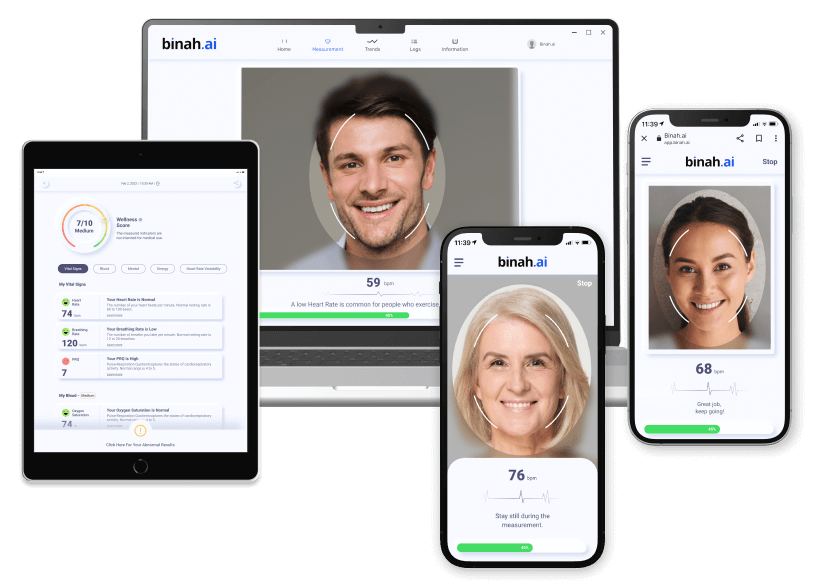
\includegraphics[scale=0.4]{Figures/binah.png}
    \caption{application binah}
    \label{fig:binah_app}
\end{figure}

\textbf{VitalSigns  Philips} constitue une solution hospitalière robuste. Intégrée dans les systèmes de surveillance médicale, elle permet un monitoring continu des patients sans contact. Cette solution excelle dans les environnements cliniques contrôlés mais n'est pas adaptée aux applications grand public en raison de sa complexité et de son coût prohibitif.

\begin{figure}[H]
    \centering
    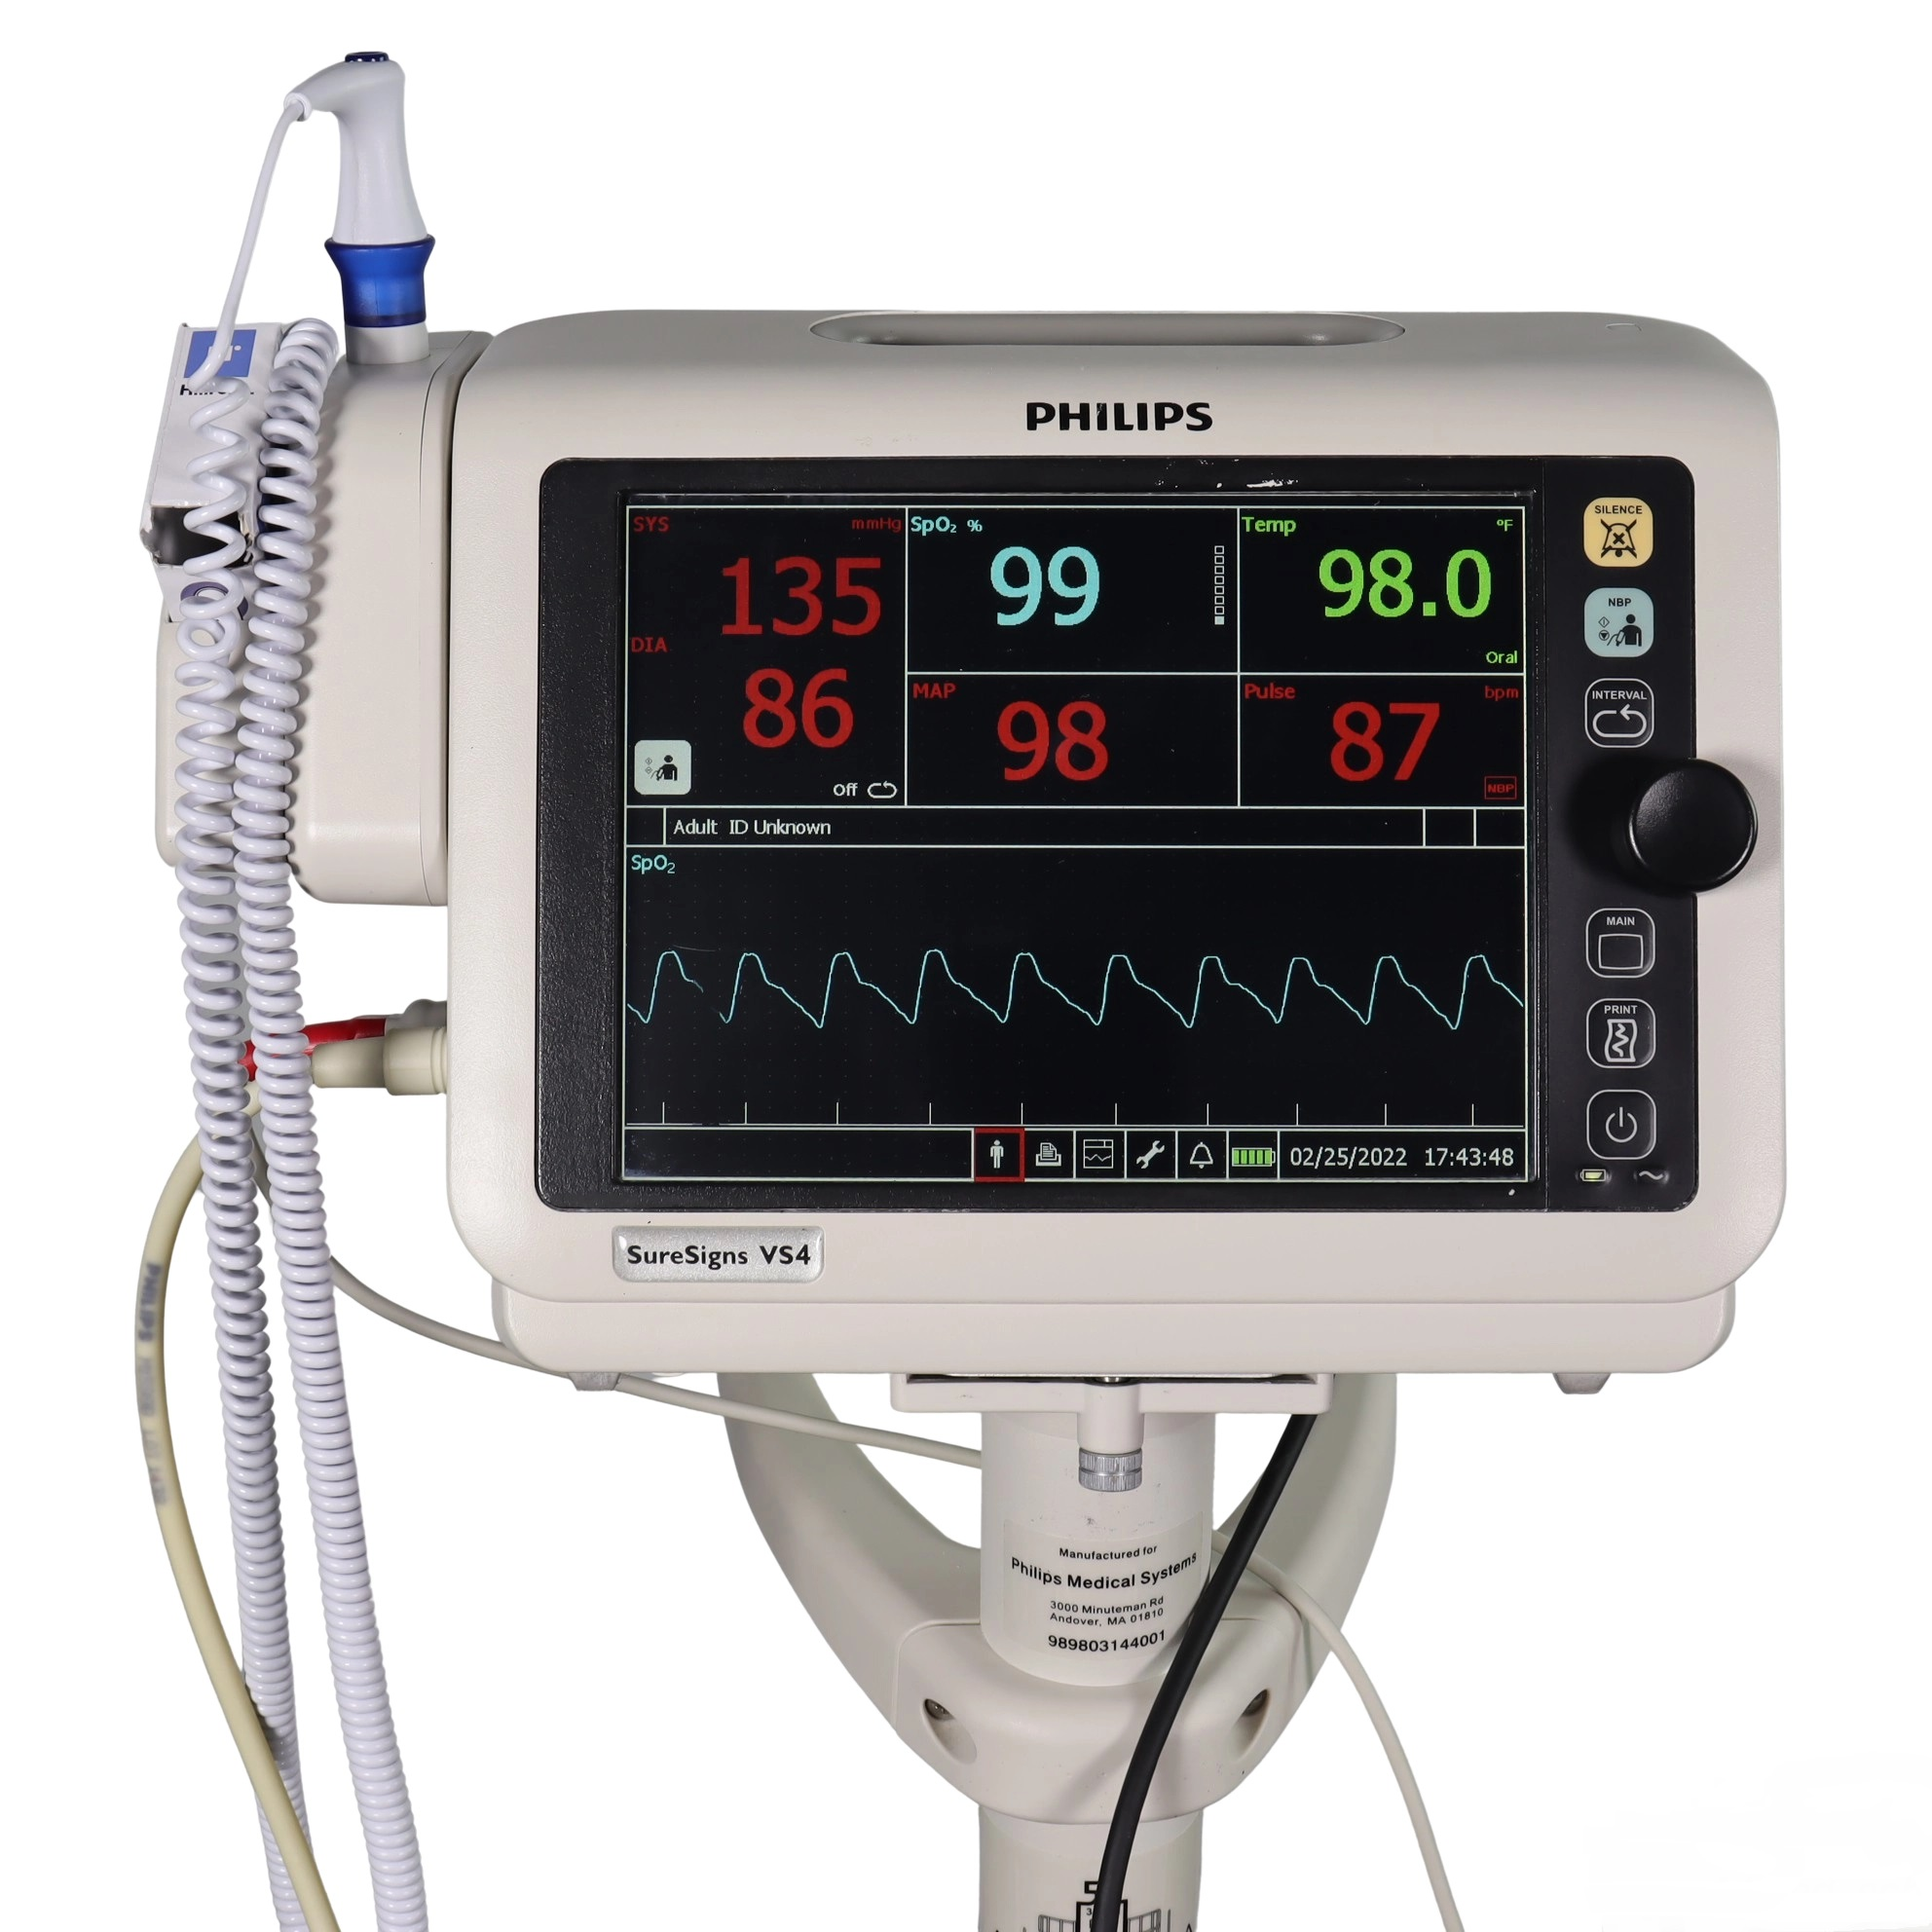
\includegraphics[scale=0.1]{Figures/Philips.png}
    \caption{VitalSigns  Philips}
    \label{fig:philips_vitalsigns}
\end{figure}

\subsubsection*{Tableau comparatif des solutions d'analyse des signaux vitaux}

\begin{table}[h]
\centering
\begin{tabular}{|p{2.2cm}|p{1.8cm}|p{1.8cm}|p{1.8cm}|p{2.8cm}|}
\hline
\textbf{Solution} & \textbf{Type} & \textbf{Coût} & \textbf{Précision} & \textbf{Paramètres mesurés} \\
\hline
Binah.ai & Commercial & Très élevé & Très élevée (< 3\%) & FC, FR, PA \\
\hline
VitalSigns Philips & Hospitalier & Très élevé & Très élevée & FC, FR, SpO2, PA, Température \\
\hline
\textbf{MindCare-AI} & \textbf{Intégré} & \textbf{Gratuit} & \textbf{Très Élevée} & \textbf{FC, PA, état émotionnel} \\
\hline
\end{tabular}
\caption{Comparaison des solutions d'analyse des signaux vitaux}
\label{tab:vitalsigns_comparison}
\end{table}

\textbf{Légende :}
\begin{itemize}
    \item FC : Fréquence Cardiaque 
    \item FR : Fréquence Respiratoire
    \item PA : Pression Artérielle
    \item SpO2 : Saturation en Oxygène
\end{itemize}


\subsection{Chatbots thérapeutiques}

Le domaine des chatbots thérapeutiques et d'accompagnement en santé mentale a connu une croissance exponentielle, particulièrement depuis la pandémie de COVID-19. Ces solutions visent à démocratiser l'accès aux soins psychologiques et à offrir un soutien 24/7 aux personnes en détresse.Par example

\textbf{Woebot} figure parmi les pionniers du secteur. Développé par des psychologues de Stanford, ce chatbot utilise la thérapie cognitivo-comportementale (TCC) pour aider les utilisateurs à gérer leur anxiété et leur dépression. Woebot propose des conversations structurées, des exercices de réflexion et un suivi de l'humeur. Les études cliniques montrent une efficacité significative dans la réduction des symptômes dépressifs. Cependant, Woebot présente des limitations : interactions parfois rigides, manque de personnalisation avancée, et coût d'abonnement mensuel.~\cite{woebot}
\begin{figure}[H]
    \centering
    
\includegraphics[scale=0.4]{Figures/logo.png}
    \caption{Woebot Health}
    \label{fig:woebot_health}
\end{figure}

\textbf{Replika} propose une approche différente en tant que "compagnon IA" personnalisé. Utilisant des modèles de langage avancés, Replika apprend des conversations avec l'utilisateur pour développer une personnalité unique. Bien que non spécifiquement thérapeutique, cette application offre un soutien émotionnel et une écoute active. Ses forces incluent une personnalisation poussée et des conversations naturelles, mais elle manque de fondements thérapeutiques validés scientifiquement.~\cite{replika} 

\begin{figure}[H]
    \centering
    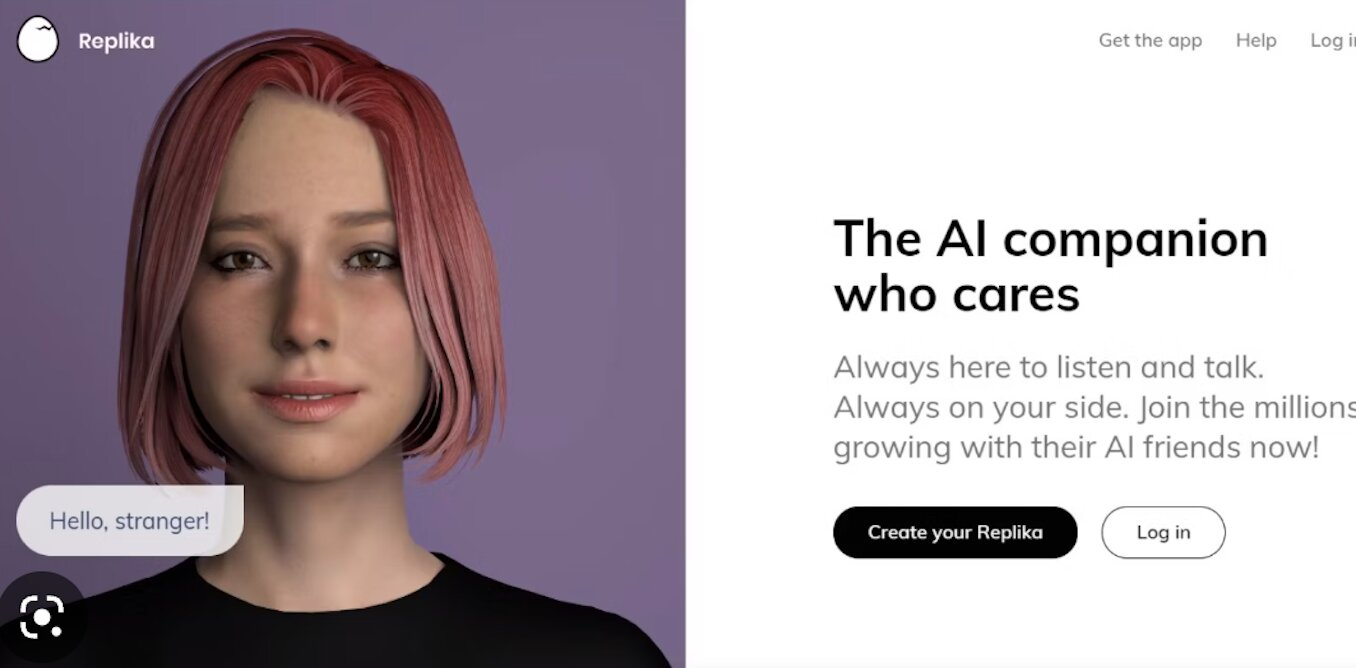
\includegraphics[scale=0.2]{Figures/replika.png}
    \caption{Replika}
    \label{fig:replika_app}
\end{figure}



\subsubsection*{Tableau comparatif des solutions de chatbots }

\begin{table}[H]
\centering
\begin{tabular}{|p{2.5cm}|p{2cm}|p{2.5cm}|p{2.5cm}|}
\hline
\textbf{Solution} & \textbf{Coût} & \textbf{Personnalisé} & \textbf{Intégration} \\
\hline
Woebot & Payant & Moyenne & Limitée \\
\hline
Replika & Payant & Élevée & Faible \\
\hline
\textbf{MindCare-AI} & \textbf{Gratuit} & \textbf{Élevée} & \textbf{Multimodale} \\
\hline
\end{tabular}
\caption{Comparaison des solutions de chatbots thérapeutiques}
\label{tab:chatbot_comparison}
\end{table}

\subsubsection*{Analyse critique et positionnement}

L'analyse de ces solutions révèle plusieurs lacunes que MindCare-AI ambitionne de combler :

\begin{itemize}
    \item \textbf{Intégration multimodale} : Aucune solution n'intègre efficacement l'analyse des signaux vitaux avec l'interaction conversationnelle
    \item \textbf{Personnalisation avancée} : La plupart des chatbots proposent des approches standardisées sans adaptation fine aux profils individuels
    \item \textbf{Accessibilité complète} : Beaucoup de solutions proposent des versions gratuites limitées ou des coûts d'abonnement élevés
    \end{itemize}
Cette analyse comparative confirme la pertinence de l'approche MindCare-AI, qui se positionne comme une solution intégrée combinant l'analyse physiologique, l'intelligence conversationnelle et l'approche thérapeutique validée, tout en maintenant une accessibilité optimale pour les utilisateurs.

\section{Solution proposée}
Pour répondre à ces défis, nous avons conçu le projet MindCare-AI comme une solution technologique complète et innovante, articulée autour de plusieurs axes complémentaires :
\begin{enumerate}
    \item \textbf{Analyse physiologique Fnon invasive par caméra} \\ 
    MindCare-AI utilise la photopléthysmographie à distance (rPPG) pour extraire, à partir d’une simple webcam, des signaux vitaux tels que la fréquence cardiaque et une estimation de la pression artérielle. Cette méthode permet de surveiller l’état physiologique de l’utilisateur sans contact, de manière discrète et confortable, et de détecter d’éventuels signes de stress ou de malaise physique.
    \item \textbf{Reconnaissance automatique des émotions} \\ 
    Le système intègre des modèles d’intelligence artificielle capables d’analyser le langage naturel (messages textuels) de l’utilisateur afin de détecter ses émotions dominantes (joie, tristesse, colère, peur). Cette analyse permet de mieux comprendre l’état psychologique du patient et d’identifier rapidement les situations à risque ou les changements d’humeur.
    \item \textbf{Chatbot thérapeutique interactif} \\ 
    MindCare-AI propose un agent conversationnel intelligent, accessible 24/7, qui dialogue avec l’utilisateur, pose des questions d’auto-évaluation validées cliniquement, évalue le niveau de stress, et fournit des conseils personnalisés. Le chatbot peut également proposer des exercices de relaxation, des recommandations de musicothérapie .
    \item \textbf{Suivi personnalisé et recommandations adaptatives} \\ 
    Le système combine les données physiologiques et émotionnelles pour offrir un suivi global et contextualisé. Il adapte ses recommandations en fonction de l’évolution de l’état de l’utilisateur, détecte précocement les signaux d’alerte, et permet un accompagnement continu, même en dehors des consultations médicales traditionnelles.
    \item \textbf{Accessibilité, sécurité et respect de la vie privée} \\ 
    MindCare-AI est conçu pour être accessible via smartphones, sans nécessiter de matériel médical spécifique. Les données sont traitées de manière sécurisée et confidentielle, dans le respect des réglementations en vigueur.
\end{enumerate}

En résumé, avec MindCare-AI, nous ambitionnons de démocratiser l’accès au suivi de la santé mentale, de faciliter la prévention et la détection précoce des troubles, et d’offrir un accompagnement personnalisé, réactif et non invasif, adapté aux besoins de chaque utilisateur. Grâce à l’intégration de l’IA, de l’analyse physiologique et d’un chatbot thérapeutique, notre projet vise à améliorer la qualité de vie et le bien-être des patients .
\section{Méthodologie du projet}

La réussite d'un projet repose en grande partie sur la méthodologie choisie pour sa conduite. Une approche méthodologique rigoureuse favorise une progression structurée, une meilleure gestion des imprévus et l'assurance de livrables de qualité. 

Dans le contexte de ce projet, qui associe le développement d'une application mobile et la mise en œuvre de modèles d'intelligence artificielle, il est primordial d'adopter des méthodologies adaptées à chaque domaine. Ainsi, deux approches complémentaires et imbriquées ont été retenues : 

\begin{itemize}
    \item L'approche \textbf{Agile avec Scrum} pour le développement logiciel de l'application
    \item La méthodologie \textbf{CRISP-DM} pour les aspects relevant de la Data Science et de l'IA
\end{itemize}

Cette approche hybride permet de bénéficier des avantages spécifiques de chaque méthodologie tout en maintenant une cohérence globale dans la gestion du projet.

\subsection{Méthodologie suivie pour le développement logiciel}

La méthode Scrum repose sur une organisation du travail en cycles courts et itératifs, appelés \textit{sprints}, d’une durée généralement comprise entre deux et quatre semaines. Au début de chaque sprint, nous avons défini un ensemble de tâches prioritaires à réaliser (le \textit{backlog}), en tenant compte des objectifs du projet et des retours obtenus lors des phases précédentes.

Chaque sprint s’est conclu par une revue permettant d’évaluer les fonctionnalités développées, de recueillir les retours des parties prenantes et d’ajuster la planification pour le sprint suivant. Cette organisation itérative nous a permis d’assurer une progression régulière du projet, d’intégrer progressivement les différentes fonctionnalités (analyse physiologique, reconnaissance des émotions, chatbot, etc.) et d’améliorer continuellement la qualité de la solution.

\begin{figure}[H]
    \centering
    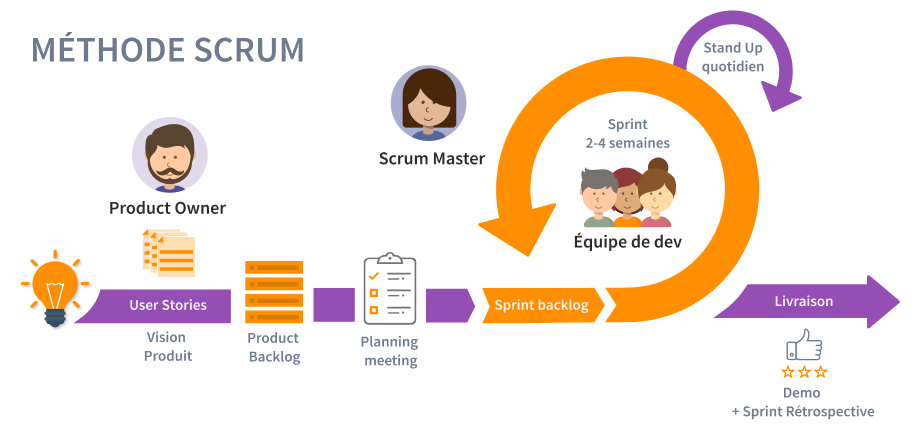
\includegraphics[scale=0.4]{Figures/Scrum.jpg}
    \caption{Processus Scrum}
    \label{fig:scrum}
\end{figure}
\newpage

Les principales étapes du processus Scrum sont les suivantes :

\begin{description}
    \item[\textbf{Product Backlog}] L’ensemble des fonctionnalités, améliorations et corrections à développer est recensé dans le product backlog. Cette liste est priorisée par le Product Owner en fonction des objectifs du projet et des besoins des utilisateurs.
    \item[\textbf{Planification du Sprint}] Au début de chaque sprint, l’équipe sélectionne les éléments du product backlog à réaliser pendant le sprint. Ces éléments constituent le sprint backlog.
    \item[\textbf{Exécution du Sprint}] L’équipe de développement travaille de manière collaborative pour implémenter les fonctionnalités sélectionnées. Des réunions quotidiennes (\textit{daily Scrum}) permettent de suivre l’avancement, de discuter des obstacles et d’ajuster les tâches si nécessaire.
    \item[\textbf{Revue de Sprint}] À la fin du sprint, l’équipe présente le travail accompli aux parties prenantes. Les retours sont recueillis afin d’améliorer le produit et le processus.
    \item[\textbf{Rétrospective du Sprint}] L’équipe analyse ce qui a bien fonctionné, ce qui peut être amélioré, et définit des actions pour optimiser le sprint suivant.
\end{description}

\subsection{Méthodologie pour la partie IA}

Pour la partie intelligence artificielle du projet MindCare-AI, la méthodologie \textbf{CRISP-DM} (Cross-Industry Standard Process for Data Mining) a été adoptée. Cette approche structurée et itérative est particulièrement adaptée aux projets de Data Science et d’IA. Elle a guidé le développement aussi bien du module d’analyse des signes vitaux que du module chatbot. Voici comment les étapes ont été appliquées :

\begin{enumerate}
    \item \textbf{Compréhension du métier} : Définition des objectifs du projet, tels que l’estimation automatisée des signes vitaux (fréquence cardiaque, pression artérielle) à partir d’images faciales, et la mise en place d’un chatbot conversationnel pour l’accompagnement psychologique et la recommandation personnalisée.
    \item \textbf{Compréhension des données} : Analyse des sources de données utilisées pour l’entraînement des modèles (par exemple, la base PPG-DaLiA pour les signes vitaux, corpus de dialogues pour le chatbot), compréhension des variables démographiques et des signaux physiologiques extraits des images, ainsi que des intentions et émotions dans les conversations.
    \item \textbf{Préparation des données} : Prétraitement des images (décodage, détection du visage, extraction des régions d’intérêt), extraction de caractéristiques pertinentes (features temporelles, fréquentielles et démographiques), normalisation et sélection des variables pour l’IA. Pour le chatbot, nettoyage et structuration des données textuelles, annotation des émotions et des intentions.
    \item \textbf{Modélisation} : Entraînement de modèles de classification supervisée (Gradient Boosting pour les signes vitaux, modèles de deep learning pour la détection d’émotions), intégration de modèles de langage (LLM) pour le chatbot, et validation croisée pour optimiser la performance.
    \item \textbf{Évaluation} : Validation des modèles sur des jeux de données tests, mesure de la précision, du rappel et du score F1 pour l’IA, et analyse de la pertinence et de la qualité des réponses pour le chatbot.
    \item \textbf{Déploiement} : Intégration des modèles entraînés dans l’API Flask du projet : le modèle d’analyse des signes vitaux est utilisé en temps réel pour traiter les images envoyées par les utilisateurs, tandis que le chatbot gère les conversations, l’évaluation du stress et la recommandation musicale personnalisée.
\end{enumerate}

La figure suivante illustre les différentes étapes de la méthodologie CRISP-DM appliquées à MindCare-AI.

\begin{figure}[H]
    \centering
    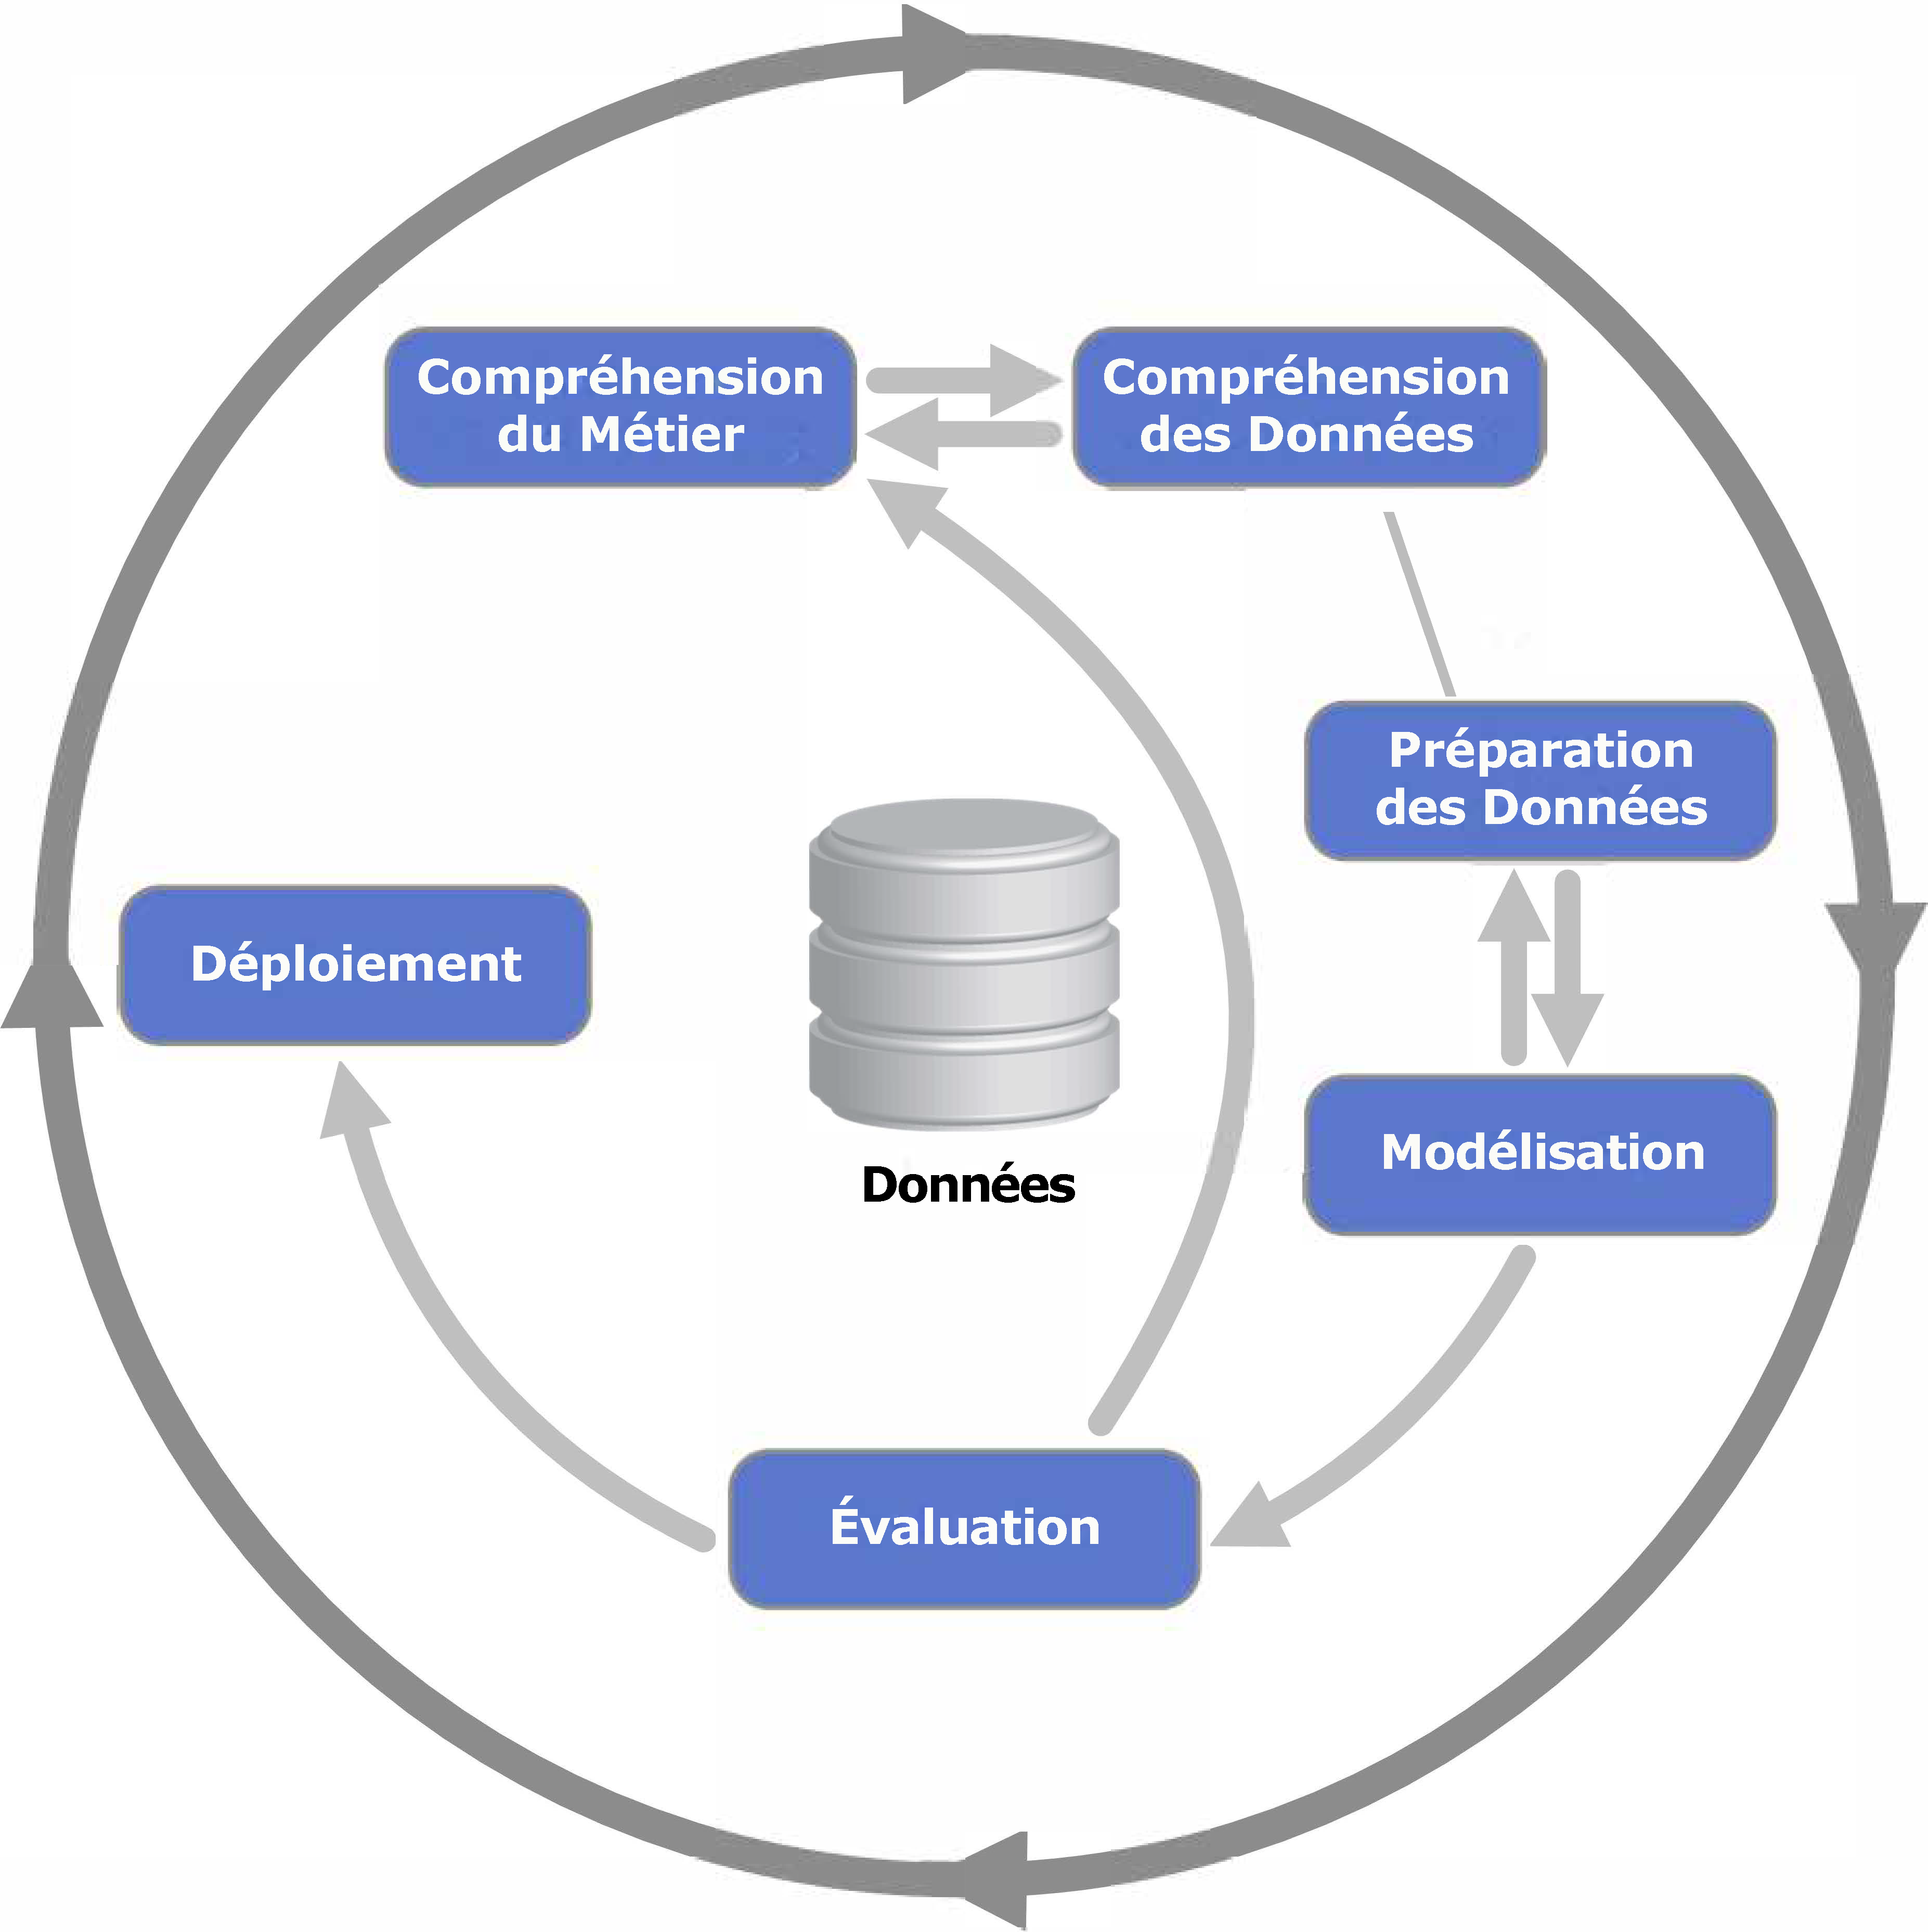
\includegraphics[width=0.8\textwidth]{Figures/Diagramme_du_Processus_CRISP-DM.png}
    \caption{Méthodologie CRISP-DM }
\end{figure}


\section{Conclusion}

En conclusion, ce chapitre a permis d’établir le cadre général du projet MindCare-AI. Nous avons présenté la société d’accueil, exposé le contexte et les enjeux liés à la santé mentale, puis formulé la problématique à laquelle nous avons souhaité répondre. Nous avons également détaillé la solution innovante proposée, en mettant en avant ses différents axes, et expliqué les méthodologies adoptées pour mener à bien le projet. Ces éléments constituent les fondations nécessaires à la compréhension des choix techniques et organisationnels qui seront approfondis dans les chapitres suivants.
\chapter{Initialisation du projet}
\begingroup
\etocsettocstyle{\rule{\linewidth}{\tocrulewidth}\vskip0.5\baselineskip}{\rule{\linewidth}{\tocrulewidth}}
\localtableofcontents
\endgroup
\newpage

\section{Introduction}
Après avoir établi le contexte général de notre projet dans le chapitre précédent, ce chapitre marque le passage de la vision stratégique à la planification opérationnelle de MindCare-AI. Il pose les fondations méthodologiques et techniques en définissant précisément le périmètre fonctionnel, les acteurs impliqués, ainsi que les exigences de qualité qui guideront l'ensemble du développement.

Nous présentons d'abord l'analyse des besoins qui identifie les utilisateurs cibles et spécifie leurs attentes fonctionnelles et non fonctionnelles. Ensuite, nous détaillons l'écosystème technologique soigneusement sélectionné pour garantir performance, évolutivité et maintenabilité. Enfin, nous structurons le travail à travers un Product Backlog hiérarchisé et une planification stratégique.

\section{Analyse des besoins}

\subsection{Identification des acteurs}
Notre analyse a permis d'identifier les acteurs principaux du système :
\begin{itemize}
    \item \textbf{Utilisateur} : Acteur principal qui surveille sa santé mentale, capture des images faciales pour l'analyse rPPG, interagit avec l'assistant conversationnel, consulte son historique et reçoit des recommandations personnalisées.
    \item \textbf{Système IA} : Ensemble des modules d'intelligence artificielle (rPPG, détection émotionnelle, chatbot adaptatif) qui analysent les données et génèrent des recommandations.
\end{itemize}

\subsection{Spécification des besoins}

\subsubsection{Besoins fonctionnels }
\begin{itemize}
    \item \textbf{Authentification et gestion de profil}
    \begin{itemize}
        \item Créer un compte sécurisé avec validation email
        \item Se connecter via authentification JWT
        \item Gérer les informations démographiques de base
    \end{itemize}
    
    \item \textbf{Analyse des signes vitaux}
    \begin{itemize}
        \item Capturer une image faciale via la caméra du smartphone
        \item Déclencher l'analyse rPPG pour estimation de la fréquence cardiaque
        \item Visualiser les résultats d'analyse en temps réel
        \item Consulter l'historique des mesures effectuées
    \end{itemize}
    
    \item \textbf{Accompagnement conversationnel}
    \begin{itemize}
        \item Dialoguer avec l'assistant intelligent empathique
        \item Recevoir des réponses adaptées à l'état émotionnel détecté
        \item Consulter l'historique des conversations
        \item Bénéficier d'un suivi contextuel des échanges
    \end{itemize}
    
    \item \textbf{Suivi et visualisations}
    \begin{itemize}
        \item Consulter les tableaux de bord (qualité du sommeil, niveau de stress, temps d'usage)
        \item Accéder aux statistiques hebdomadaires et mensuelles
    \end{itemize}
    
    \item \textbf{Recommandations personnalisées}
    \begin{itemize}
        \item Recevoir des suggestions de musique adaptées à l'état émotionnel
        \item Obtenir des conseils de bien-être basés sur l'analyse multimodale
   \end{itemize}
\end{itemize}
\subsubsection{Besoins non fonctionnels}
Les exigences de qualité identifiées pour assurer une expérience utilisateur optimale :
\begin{itemize}
    \item \textbf{Sécurité et confidentialité} : Protection stricte des données personnelles et médicales conformément aux réglementations en vigueur, avec chiffrement des communications et stockage sécurisé.
    \item \textbf{Performance temps réel} : Les analyses d'IA (détection d'émotions, estimation rPPG) s'exécutent en moins de 7 secondes pour garantir une expérience fluide et engageante.
    \item \textbf{Compatibilité multiplateforme} : L'application fonctionne de manière native sur les principaux systèmes mobiles (Android, iOS) avec une interface adaptative.
    \item \textbf{Évolutivité} : L'architecture modulaire permet l'ajout de nouvelles fonctionnalités d'IA et le passage à l'échelle pour un grand nombre d'utilisateurs.
    \item \textbf{Ergonomie intuitive} : Interface utilisateur moderne et accessible, conçue pour tous les profils d'âge et de compétence technologique.
\end{itemize}

\section{Technologies et outils utilisés}
Le développement de MindCare-AI s'appuie sur un écosystème technologique soigneusement sélectionné pour optimiser les performances, la maintenabilité et l'évolutivité du système. Les tableaux suivants présentent l'ensemble des technologies et outils utilisés, organisés par domaine d'application.

\begin{table}[H]\centering
\small
\renewcommand{\arraystretch}{2.5}
\begin{tabularx}{\linewidth}{|p{3cm}|>{\centering\arraybackslash}p{4cm}|>{\centering\arraybackslash}X|}
\hline
\textbf{Domaine} & \textbf{Technologie/Outil} & \textbf{Description} \\
\hline
\multicolumn{3}{|l|}{\textbf{Langages de Programmation}}\\
\hline
 Backend & 
\begin{minipage}[c]{4cm}
\centering

\includegraphics[width=2cm,height=1.2cm]{Figures/technologie/js.png}
\end{minipage}
& 
\begin{minipage}[c]{\linewidth}
\centering
Langage de programmation dynamique pour applications web et mobiles~\cite{javaScript}.
\end{minipage} \\
\hline
Frontend & 
\begin{minipage}[c]{4cm}
\centering

\includegraphics[width=2cm,height=1.2cm]{Figures/technologie/ts.png}
\end{minipage}
& 
\begin{minipage}[c]{\linewidth}
\centering
Surcouche typée de JavaScript pour améliorer la robustesse du code~\cite{typescript}.
\end{minipage} \\
\hline
IA & 
\begin{minipage}[c]{4cm}
\centering

\includegraphics[width=2cm,height=1.2cm]{Figures/technologie/Python.png}
\end{minipage}
& 
\begin{minipage}[c]{\linewidth}
\centering
Langage spécialisé en science des données et intelligence artificielle~\cite{python}.
\end{minipage} \\
\hline
\multicolumn{3}{|l|}{\textbf{Frontend Mobile}}\\
\hline
Framework & 
\begin{minipage}[c]{4cm}
\centering

\includegraphics[width=2cm,height=1.2cm]{Figures/technologie/react native.png}
\end{minipage}
& 
\begin{minipage}[c]{\linewidth}
\centering
Framework multiplateforme pour développement d'applications natives~\cite{react_native}.
\end{minipage} \\
\hline
Plateforme & 
\begin{minipage}[c]{4cm}
\centering

\includegraphics[width=2cm,height=1.2cm]{Figures/technologie/expo.png}
\end{minipage}
& 
\begin{minipage}[c]{\linewidth}
\centering
Plateforme de développement React Native avec déploiement simplifié~\cite{expo}.
\end{minipage} \\
\hline
Navigation & 
\begin{minipage}[c]{4cm}
\centering

\includegraphics[width=2cm,height=1.2cm]{Figures/technologie/react navigation.png}
\end{minipage}
& 
\begin{minipage}[c]{\linewidth}
\centering
Bibliothèque de navigation avec animations fluides pour applications mobiles~\cite{react_navigation}.
\end{minipage} \\
\hline
\multicolumn{3}{|l|}{\textbf{Backend Principal}}\\
\hline
Runtime & 
\begin{minipage}[c]{4cm}
\centering

\includegraphics[width=2cm,height=1.2cm]{Figures/technologie/node.jpeg}
\end{minipage}
& 
\begin{minipage}[c]{\linewidth}
\centering
Environnement d'exécution JavaScript haute performance côté serveur~\cite{nodejs}.
\end{minipage} \\
\hline
Framework & 
\begin{minipage}[c]{4cm}
\centering

\includegraphics[width=2cm,height=1.2cm]{Figures/technologie/express.jpg}
\end{minipage}
& 
\begin{minipage}[c]{\linewidth}
\centering
Framework web minimaliste et flexible pour création d'APIs REST~\cite{express}.
\end{minipage} \\
\hline
Authentification & 
\begin{minipage}[c]{4cm}
\centering

\includegraphics[width=2cm,height=1.2cm]{Figures/technologie/jwt.png}
\end{minipage}
& 
\begin{minipage}[c]{\linewidth}
\centering
Tokens sécurisés pour authentification utilisateur sans état~\cite{jwt}.
\end{minipage} \\
\hline
\end{tabularx}
\end{table}

\begin{table}[H]\centering
\small
\renewcommand{\arraystretch}{2.5}
\begin{tabularx}{\linewidth}{|p{3cm}|>{\centering\arraybackslash}p{4cm}|>{\centering\arraybackslash}X|}
\hline
\multicolumn{3}{|l|}{\textbf{Backend IA Spécialisé}}\\
\hline
Framework & 
\begin{minipage}[c]{4cm}
\centering
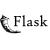
\includegraphics[width=2cm,height=1.2cm]{Figures/technologie/flask.png}
\end{minipage}
& 
\begin{minipage}[c]{\linewidth}
\centering
Micro-framework web Python léger pour modules d'intelligence artificielle~\cite{flask}.
\end{minipage} \\
\hline
ML/DL & 
\begin{minipage}[c]{4cm}
\centering

\includegraphics[width=2cm,height=1.2cm]{Figures/technologie/tensorflow.png}
\end{minipage}
& 
\begin{minipage}[c]{\linewidth}
\centering
Plateforme open-source d'apprentissage automatique ~\cite{tensorflow}.
\end{minipage} \\
\hline
ML/DL & 
\begin{minipage}[c]{4cm}
\centering

\includegraphics[width=2cm,height=1.2cm]{Figures/technologie/sklearn.png}
\end{minipage}
& 
\begin{minipage}[c]{\linewidth}
\centering
Bibliothèque Python complète pour apprentissage automatique et classification~\cite{scikit_learn}.
\end{minipage} \\
\hline
Traitement & 
\begin{minipage}[c]{4cm}
\centering

\includegraphics[width=2cm,height=1.2cm]{Figures/technologie/opencv.png}
\end{minipage}
& 
\begin{minipage}[c]{\linewidth}
\centering
Bibliothèque de vision par ordinateur pour détection faciale et analyse d'images~\cite{opencv}.
\end{minipage} \\
\hline
NLP & 
\begin{minipage}[c]{4cm}
\centering

\includegraphics[width=2cm,height=1.2cm]{Figures/technologie/transformers.png}
\end{minipage}
& 
\begin{minipage}[c]{\linewidth}
\centering
Bibliothèque de modèles pré-entraînés pour traitement du langage naturel~\cite{transformers}.
\end{minipage} \\
\hline
Calcul & 
\begin{minipage}[c]{4cm}
\centering

\includegraphics[width=2cm,height=1.2cm]{Figures/technologie/numpy.png}
\end{minipage}
& 
\begin{minipage}[c]{\linewidth}
\centering
Bibliothèque de calcul scientifique Python pour traitement de signaux numériques~\cite{numpy}.
\end{minipage} \\
\hline
Données & 
\begin{minipage}[c]{4cm}
\centering

\includegraphics[width=2cm,height=1.2cm]{Figures/technologie/pandas.png}
\end{minipage}
& 
\begin{minipage}[c]{\linewidth}
\centering
Bibliothèque Python de manipulation et analyse de données structurées~\cite{pandas}.
\end{minipage} \\
\hline
\multicolumn{3}{|l|}{\textbf{Base de Données}}\\
\hline
SGBD & 
\begin{minipage}[c]{4cm}
\centering

\includegraphics[width=2cm,height=1.2cm]{Figures/technologie/mongodb.png}
\end{minipage}
& 
\begin{minipage}[c]{\linewidth}
\centering
Base de données NoSQL orientée documents pour flexibilité des schémas~\cite{mongodb}.
\end{minipage} \\
\hline
\multicolumn{3}{|l|}{\textbf{Développement et Outils}}\\
\hline
Versioning & 
\begin{minipage}[c]{4cm}
\centering

\includegraphics[width=2cm,height=1.2cm]{Figures/technologie/git.png}
\end{minipage}
& 
\begin{minipage}[c]{\linewidth}
\centering
Système de contrôle de version distribué pour collaboration en équipe~\cite{git}.
\end{minipage} \\
\hline
IDE & 
\begin{minipage}[c]{4cm}
\centering

\includegraphics[width=2cm,height=1.2cm]{Figures/technologie/vscode.jpeg}
\end{minipage}
& 
\begin{minipage}[c]{\linewidth}
\centering
Éditeur de code source extensible avec support multi-langages~\cite{vscode}.
\end{minipage} \\
\hline
Tests API & 
\begin{minipage}[c]{4cm}
\centering

\includegraphics[width=2cm,height=1.2cm]{Figures/technologie/postman.png}
\end{minipage}
& 
\begin{minipage}[c]{\linewidth}
\centering
Plateforme complète de test, documentation et collaboration pour APIs~\cite{postman}.
\end{minipage} \\
\hline
Design & 
\begin{minipage}[c]{4cm}
\centering

\includegraphics[width=2cm,height=1.2cm]{Figures/technologie/figma.png}
\end{minipage}
& 
\begin{minipage}[c]{\linewidth}
\centering
Outil de conception d'interfaces utilisateur collaboratif basé sur le cloud~\cite{figma}.
\end{minipage} \\
\hline
IA Locale & 
\begin{minipage}[c]{4cm}
\centering
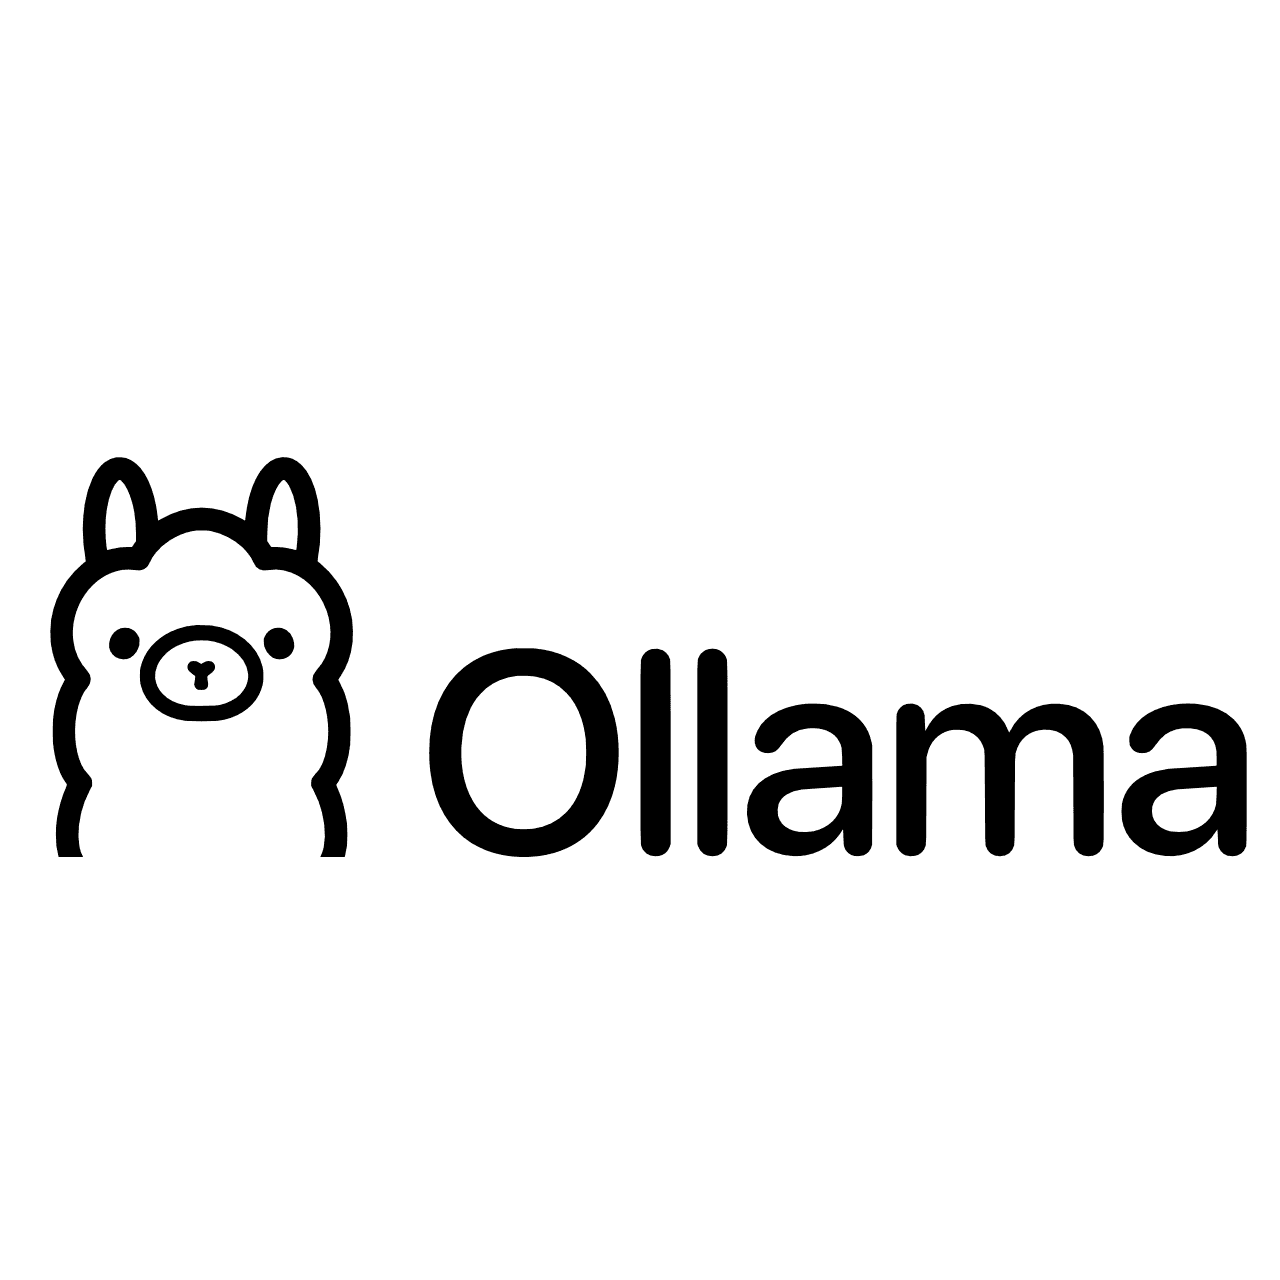
\includegraphics[width=2cm,height=1.2cm]{Figures/technologie/ollama.png}
\end{minipage}
& 
\begin{minipage}[c]{\linewidth}
\centering
Plateforme d'exécution locale de modèles LLM pour développement et test d'IA~\cite{ollama}.
\end{minipage} \\

\hline
\end{tabularx}
\end{table}

\begin{table}[H]\centering
\small
\renewcommand{\arraystretch}{2.5}
\begin{tabularx}{\linewidth}{|p{3cm}|>{\centering\arraybackslash}p{4cm}|>{\centering\arraybackslash}X|}
\hline
\multicolumn{3}{|l|}{\textbf{Documentation et Rédaction}}\\
\hline
Rédaction & 
\begin{minipage}[c]{4cm}
\centering

\includegraphics[width=2cm,height=1.2cm]{Figures/technologie/latex.png}
\end{minipage}
& 
\begin{minipage}[c]{\linewidth}
\centering
Système de composition de documents pour la rédaction scientifique et académique~\cite{latex}.
\end{minipage} \\
\hline
Diagrammes & 
\begin{minipage}[c]{4cm}
\centering

\includegraphics[width=2cm,height=1.2cm]{Figures/technologie/drawio.png}
\end{minipage}
& 
\begin{minipage}[c]{\linewidth}
\centering
Outil de création de diagrammes et schémas techniques pour l'architecture système~\cite{drawio}.
\end{minipage} \\
\hline
\end{tabularx}
\caption{Technologies et outils utilisés dans MindCare-AI}
\end{table}

\section{Product Backlog}
Notre Product Backlog structure le développement autour de la création de valeur utilisateur progressive, avec une approche qui privilégie d'abord la mise en place du socle applicatif, puis l'enrichissement par l'intelligence artificielle.

\begin{table}[H]\centering
\small
\renewcommand{\arraystretch}{1.12}
\begin{tabularx}{\linewidth}{|p{0.8cm}|p{3.2cm}|p{2.3cm}|X|p{1.6cm}|}
\hline
\textbf{ID} & \textbf{Épic} & \textbf{Acteur} & \textbf{Description} & \textbf{Priorité} \\
\hline
\multicolumn{5}{|l|}{\textbf{Release 1 : Application Mobile Fonctionnelle}}\\
\hline
\multicolumn{5}{|l|}{\textit{Sprint 1 : Fondations et authentification}}\\
\hline
1 & Authentification sécurisée & Utilisateur & Créer un compte, se connecter de manière sécurisée (JWT) et personnaliser son profil avec données démographiques. & Haute \\
\hline
\multicolumn{5}{|l|}{\textit{Sprint 2 : Interface utilisateur moderne}}\\
\hline
2 & Interface principale & Utilisateur & Accéder à un tableau de bord personnalisé et naviguer intuitivement vers toutes les fonctionnalités. & Haute \\
\hline
3 & Auto-évaluations mentales & Utilisateur & Compléter des questionnaires de bien-être et suivre l'évolution de ses états émotionnels. & Moyenne \\
\hline
\multicolumn{5}{|l|}{\textit{Sprint 3 : Assistant conversationnel}}\\
\hline
4 & Assistant conversationnel & Utilisateur & Dialoguer avec un chatbot empathique et conserver l'historique des échanges pour un suivi personnalisé. & Haute \\
\hline
5 & Recommandations de base & Utilisateur & Recevoir des suggestions musicales et des rappels personnalisés pour le bien-être. & Basse \\
\hline
\multicolumn{5}{|l|}{\textit{Sprint 4 : Interface d'analyse rPPG et visualisations}}\\
\hline
6 & Module de capture & Utilisateur & Utiliser l'interface caméra avec détection faciale pour préparer l'analyse des signes vitaux. & Haute \\
\hline
7 & Historique et visualisations & Utilisateur & Consulter l'évolution de ses métriques et visualiser des graphiques de tendances. & Moyenne \\
\hline
\multicolumn{5}{|l|}{\textbf{Release 2 : Intelligence Artificielle Avancée}}\\
\hline
\multicolumn{5}{|l|}{\textit{Sprint 1 : Analyse rPPG des signes vitaux}}\\
\hline
8 & Analyse rPPG intelligente & Système IA & Estimer avec précision les signes vitaux (fréquence cardiaque, pression artérielle) à partir d'images faciales via des modèles d'apprentissage automatique optimisés. & Haute \\
\hline
9 & Validation et robustesse & Système IA & Valider les performances du modèle rPPG sur différents profils utilisateurs et conditions d'éclairage. & Haute \\
\hline
\end{tabularx}
\end{table}


\begin{table}[H]\centering
\small
\renewcommand{\arraystretch}{1.12}
\begin{tabularx}{\linewidth}{|p{0.8cm}|p{3.2cm}|p{2.3cm}|X|p{1.6cm}|}
\hline
\multicolumn{5}{|l|}{\textit{Sprint 2 : Chatbot émotionnel adaptatif}}\\
\hline
10 & Détection d'émotions & Système IA & Identifier automatiquement les émotions dans les textes conversationnels pour personnaliser les interactions. & Haute \\
\hline
11 & Chatbot adaptatif & Utilisateur & Bénéficier de réponses conversationnelles empathiques adaptées à l'état émotionnel détecté. & Haute \\
\hline
12 & Recommandations contextuelles & Utilisateur & Recevoir des suggestions personnalisées (musique, exercices, ressources) basées sur l'analyse émotionnelle et les signes vitaux. & Moyenne \\
\hline
\end{tabularx}
\caption{Product Backlog orienté valeur utilisateur avec mapping des sprints}
\end{table}

\section{Conclusion}
Ce chapitre d'initialisation a établi les fondations essentielles du projet MindCare-AI en clarifiant le périmètre fonctionnel, les acteurs impliqués et les exigences de qualité à respecter. L'analyse approfondie des besoins a permis de définir un cadre cohérent répondant aux enjeux de santé mentale identifiés, tandis que la sélection rigoureuse de l'écosystème technologique  garantit la capacité du système à évoluer et à performer durablement.

La planification stratégique en deux releases reflète notre approche pragmatique de livraison progressive de valeur : construire d'abord une application mobile complète et opérationnelle qui apporte une réelle utilité aux utilisateurs, puis l'enrichir avec des capacités d'intelligence artificielle avancées qui distingueront MindCare-AI des solutions existantes. Cette trajectoire maîtrisée, structurée autour d'un Product Backlog priorisé et de sprints bien définis, assure une progression cohérente vers notre objectif d'une application innovante d'accompagnement en santé mentale.

Le chapitre suivant approfondira les aspects organisationnels et architecturaux en présentant la méthodologie de gestion de projet Scrum adoptée ainsi que le modèle d'architecture hybride retenu pour transformer ces exigences en un système robuste, évolutif et maintenable.
\chapter{Analyse et spécification des besoins}
\begingroup
\etocsettocstyle{\rule{\linewidth}{\tocrulewidth}\vskip0.5\baselineskip }{\rule{\linewidth}{\tocrulewidth}}
\localtableofcontents
\endgroup
\newpage
\section{Introduction}
 Après avoir défini le périmètre fonctionnel et établi la planification stratégique dans le chapitre précédent, nous abordons maintenant la phase d'analyse et de spécification technique qui transforme les besoins identifiés en architecture logicielle concrète. Ce chapitre constitue le pont essentiel entre les exigences métier et l'implémentation technique, en structurant notre vision à travers des modèles architecturaux et des diagrammes UML précis.

Nous présentons d'abord l'architecture logicielle retenue, basée sur le pattern MVC qui sépare clairement les responsabilités tout en facilitant l'intégration des modules d'intelligence artificielle. Ensuite, nous détaillons l'architecture globale du système avec ses composants principaux et leurs interactions. Enfin, nous formalisons la conception détaillée à travers une modélisation UML complète incluant diagrammes de cas d'utilisation et diagramme de classes, offrant ainsi une vision structurée et partagée qui guidera l'implémentation des releases .
\section{Architecture logicielle}
Nous avons opté pour le modèle d'architecture \textbf{MVC}  qui nous permet de structurer clairement notre application en séparant les responsabilités. Cette approche s'avère particulièrement adaptée à notre contexte de développement mobile avec modules d'IA intégrés.

\subsection{Architecture MVC}
\begin{itemize}
    \item \textbf{Modèle (Model)} : Gère toutes les données de l'application (profils utilisateurs, mesures physiologiques, historique des conversations, résultats d'analyses IA) et orchestre l'accès à la base de données MongoDB.
    \item \textbf{Vue (View)} : Représente l'interface utilisateur React Native, incluant les écrans d'authentification, le tableau de bord personnalisé, l'interface de chat avec l'assistant, et les visualisations de données.
    \item \textbf{Contrôleur (Controller)} : Coordonne les interactions entre la vue et le modèle, traite les requêtes utilisateur, sollicite les modules d'IA (rPPG, détection d'émotions, recommandations) et formate les réponses.
\end{itemize}

\subsection{Flux d'interaction }
Le parcours utilisateur s'articule autour de ce modèle : l'utilisateur interagit avec la \textbf{Vue} mobile pour soumettre une image ou envoyer un message, le \textbf{Contrôleur} backend traite la requête en sollicitant les modules d'IA appropriés et met à jour le \textbf{Modèle}, puis les résultats personnalisés sont renvoyés à la vue pour afficher. Cette séparation claire facilite la maintenance et permet une évolution agile de chaque composant.~\cite{MVC}

\begin{figure}[H]
    \centering
    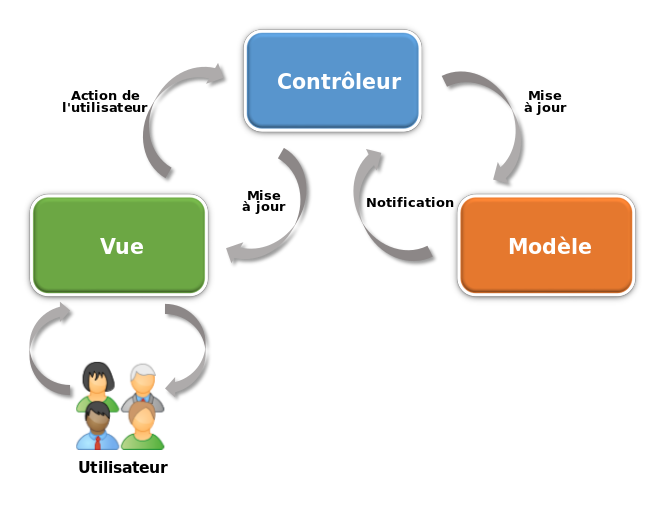
\includegraphics[width=0.8\textwidth]{Figures/Modèle–Vue–Contrôleur.png}
    \caption{Architecture MVC }
\end{figure}

\section{Architecture globale}
Notre architecture globale privilégie une approche modulaire qui sépare clairement les responsabilités tout en facilitant l'intégration harmonieuse des différents composants d'intelligence artificielle.

\subsection{Composants principaux du système}
Le système MindCare-AI s'articule autour de quatre modules principaux :
\begin{itemize}
    \item \textbf{Application mobile React Native} : Interface utilisateur moderne offrant authentification, capture d'images, chat intelligent, et visualisations personnalisées.
    \item \textbf{API REST Node.js/Express} : Serveur backend qui orchestre la logique métier, gère l'authentification JWT, coordonne les appels aux modules d'IA, et assure la persistance des données.
    \item \textbf{Modules d'intelligence artificielle }: 
    \begin{itemize}
        \item Module rPPG pour l'estimation des signes vitaux par analyse d'image faciale.
        \item Analyseur d'émotions pour la classification des sentiments dans les textes.
        \item Assistant conversationnel adaptatif avec génération de réponses empathiques.
        \item Système de recommandations personnalisées basé sur l'état psychophysiologique.
    \end{itemize}
    \item \textbf{Base de données } : Stockage sécurisé et structuré des profils utilisateurs, mesures physiologiques, conversations, et historiques d'analyses.
\end{itemize}

\subsection{Schéma d'architecture}
\begin{center}
\begin{tikzpicture}[node distance=2cm, auto]
    % Nodes
    \node[draw, rectangle, fill=blue!10] (mobile) {Application mobile};
    \node[draw, rectangle, right=4cm of mobile, fill=green!10] (backend) {Serveur backend (API REST)};
    \node[draw, rectangle, above=1.5cm of backend, fill=yellow!10, align=center] (ai) {Modules IA\\(vital\_signs, chatbot, émotions)};
    \node[draw, rectangle, below=1.5cm of backend, fill=red!10] (db) {Base de données (MongoDB)};
    % Edges
    \draw[->, thick] (mobile) -- node[above]{Requêtes API} (backend);
    \draw[->, thick] (backend) -- node[right]{Appels internes} (ai);
    \draw[->, thick] (backend) -- node[right]{Lecture/écriture} (db);
    \draw[<-, thick] (backend) -- node[below]{Réponses API} (mobile);
\end{tikzpicture}
\end{center}

\section{Conception détaillée : langage UML}
La modélisation UML nous a accompagnés tout au long de la conception pour structurer et clarifier les interactions complexes de notre système intégrant à la fois l'analyse physiologique par IA et l'accompagnement conversationnel personnalisé.~\cite{uml}

\begin{figure}[H]
    \centering
    
\includegraphics[width=0.8\textwidth]{Figures/UML_logo.png}
    \caption{ langage de modélisation unifié}
\end{figure}
\subsection{Diagramme de cas d'utilisation global}
Ce diagramme illustre l'ensemble des interactions possibles entre l'utilisateur et notre système intelligent, mettant en évidence la richesse fonctionnelle de MindCare-AI et les relations entre les différents cas d'utilisation.

\begin{figure}[H]
    \centering
    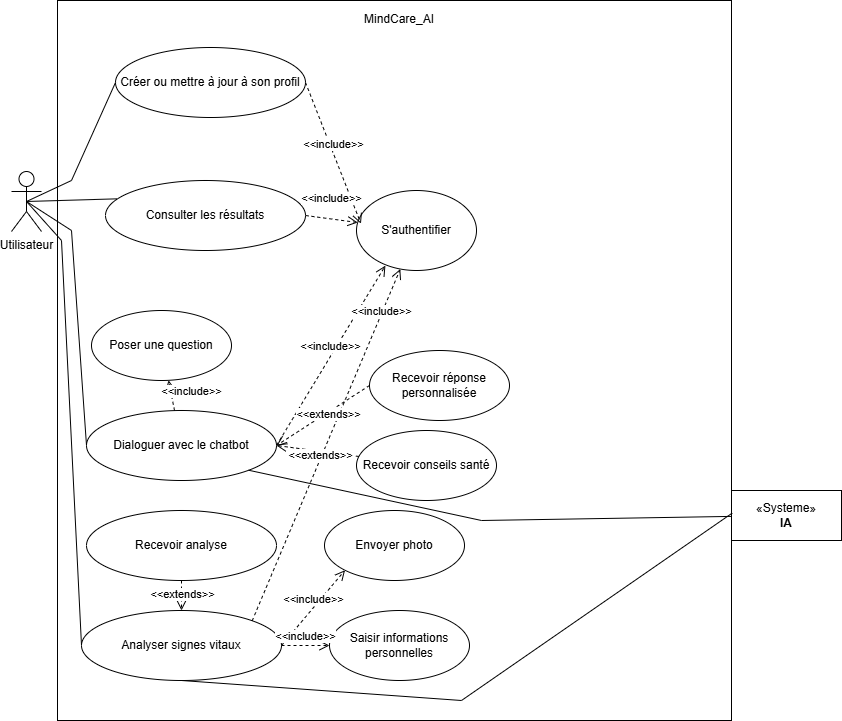
\includegraphics[width=1.1\textwidth]{Figures/useCase.png}
    \caption{Diagramme de cas d'utilisation global }
\end{figure}

\subsubsection*{Description détaillée du diagramme de cas d'utilisation}

\begin{table}[H]
\centering
\small
\begin{tabularx}{\linewidth}{|p{4cm}|X|}
\hline
\textbf{Titre} & Système MindCare-AI \\
\hline
\textbf{Acteur(s)} & Utilisateur \\
\hline
\textbf{Description} & 
Le système MindCare-AI offre un ensemble complet de fonctionnalités pour l'accompagnement en santé mentale. L'utilisateur peut gérer son profil, analyser ses signes vitaux via rPPG, dialoguer avec un assistant conversationnel empathique, consulter son historique avec visualisations, et recevoir des recommandations personnalisées de bien-être. \\
\hline
\textbf{Préconditions} & 
\begin{itemize}
    \item L'application mobile est installée sur le smartphone de l'utilisateur.
    \item L'utilisateur dispose d'une connexion internet active.
    \item Pour l'analyse rPPG : l'appareil dispose d'une caméra fonctionnelle et d'un éclairage suffisant.
\end{itemize} \\
\hline
\textbf{Postconditions} & 
\begin{itemize}
    \item L'utilisateur est authentifié et peut accéder à toutes les fonctionnalités de l'application.
    \item Toutes les données générées (analyses, conversations, évaluations) sont sauvegardées dans l'historique personnel.
    \item L'utilisateur peut consulter ses tendances et évolutions via des visualisations graphiques.
    \item Le système adapte continuellement ses recommandations en fonction de l'état psychophysiologique détecté.
\end{itemize} \\
\hline
\textbf{Scénario principal} & 
\begin{enumerate}
    \item L'utilisateur lance l'application et s'authentifie.
    \item L'utilisateur configure son profil avec ses informations personnelles.
    \item L'utilisateur accède au tableau de bord principal.
    \item L'utilisateur sélectionne une fonctionnalité (analyse des signes vitaux, dialogue avec le chatbot, ou consultation des résultats).
    \item Le système traite la demande et retourne les résultats appropriés.
    \item L'utilisateur reçoit des recommandations personnalisées selon son état détecté.
    \item Les données sont sauvegardées pour un suivi ultérieur.
\end{enumerate} \\
\hline
\end{tabularx}
\end{table}

\begin{table}[H]
\centering
\small
\begin{tabularx}{\linewidth}{|p{4cm}|X|}
\hline
\textbf{Scénarios alternatifs} & 
\begin{itemize}
    \item Échec d'authentification : affichage d'un message d'erreur et possibilité de réessayer.
    \item Problème technique (détection faciale, communication IA, connexion) : affichage d'un message d'erreur explicatif avec proposition de réessai.
    \item Données insuffisantes : le système invite l'utilisateur à effectuer une première analyse ou à compléter son profil.
    \item Résultats avec faible niveau de confiance : le système affiche un avertissement et suggère de refaire l'analyse dans de meilleures conditions.
\end{itemize} \\
\hline
\end{tabularx}
\caption{Description générale du diagramme de cas d'utilisation global}
\end{table}


Cette organisation modulaire et cohérente garantit une expérience utilisateur fluide tout en préparant l'intégration progressive des capacités d'intelligence artificielle avancées dans les releases futures.

Le parcours d'analyse des signes vitaux permet à l'utilisateur de soumettre une photo de son visage et de recevoir en retour une estimation précise de sa fréquence cardiaque et de sa pression artérielle. Le module conversationnel offre un accompagnement empathique avec un assistant capable de détecter les émotions et d'adapter ses réponses en conséquence.
\subsection{Diagramme de classe général}

Ce diagramme de classe illustre l'architecture orientée objet de MindCare-AI, centrée autour de l'entité \textbf{User} qui coordonne l'ensemble des fonctionnalités du système. L'utilisateur \textit{réalise} des évaluations psychométriques (\textbf{Assessment}) pour le suivi de son bien-être mental, et \textit{effectue} des analyses de signes vitaux (\textbf{VitalSigns}) via la technologie rPPG intégrée. Il \textit{effectue} également des conversations empathiques avec l'assistant IA (\textbf{Conversation}) qui génère des réponses personnalisées selon son état émotionnel. Le système \textit{recommande} intelligemment du contenu musical thérapeutique (\textbf{Music}) adapté au profil psychophysiologique de chaque utilisateur.

\begin{figure}[H]
    \centering
    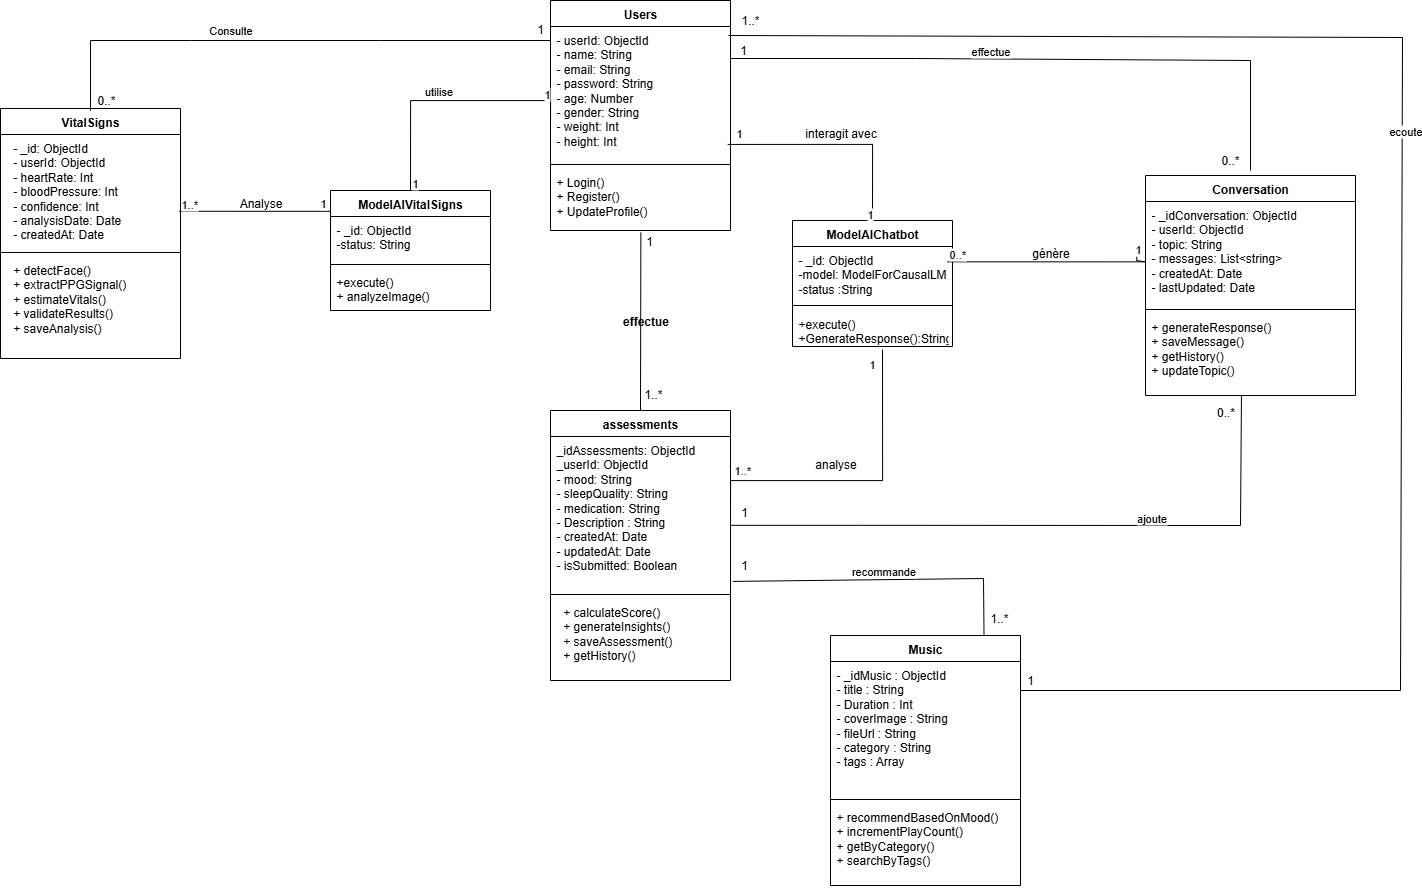
\includegraphics[angle=90, width=0.6\textheight]{Figures/class.png}
    \caption{Diagramme de classe général}
\end{figure}


\section{Conclusion}
Ce chapitre a posé les fondations architecturales et conceptuelles essentielles pour le développement de MindCare-AI. L'adoption du pattern MVC nous offre une séparation claire des responsabilités qui facilite la maintenance et l'évolution du système, tandis que l'architecture modulaire garantit une intégration harmonieuse des composants d'intelligence artificielle avec le socle applicatif.

La modélisation UML complète, incluant le diagramme de cas d'utilisation global et le diagramme de classes, constitue un référentiel de conception partagé qui assure la cohérence entre la vision fonctionnelle et l'implémentation technique. Ces modèles formalisent précisément les interactions utilisateur-système et la structure orientée objet des données, offrant ainsi une base solide pour la réalisation concrète du projet.

Le chapitre suivant entame concrètement l'implémentation de la Release 1 avec le développement progressif du socle applicatif selon la méthodologie agile définie.
\chapter{Processus global : de la compréhension des données à l’évaluation des modèles}
\newpage
\section{Introduction}
Ce chapitre est dédié à la modélisation des solutions d’intelligence artificielle intégrées dans l’application \textbf{MindCare-AI}. Il détaille le processus complet, depuis la compréhension et la préparation du dataset PPG+Dalia jusqu’à l’évaluation des modèles de classification de la fréquence cardiaque, en passant par le prétraitement des données, l’extraction de caractéristiques pertinentes, le choix des architectures adaptées, l’entraînement et l’analyse des performances.
Parallèlement, ce chapitre présente également la conception et l’intégration d’un chatbot intelligent, capable d’interagir avec les utilisateurs, de fournir des conseils personnalisés et d’exploiter les résultats des analyses physiologiques pour un accompagnement en temps réel.
L’utilisation de modèles avancés, de pipelines de prétraitement éprouvés et de techniques d’IA conversationnelle permet ainsi d’assurer à la fois une détection fiable des états physiologiques et une expérience utilisateur interactive, personnalisée et sécurisée.
\section{Collection et préparation des données}

Nous  commencons par la collection du dataset :

\subsection{Collection du jeu de données}

La première étape du processus a consisté à collecter et explorer le jeu de données adapté aux objectifs de l’application MindCare-AI. Cette phase, essentielle dans la démarche CRISP-DM, vise à comprendre la nature des données disponibles, à identifier les caractéristiques pertinentes pour l’analyse des signaux physiologiques, et à anticiper les éventuels problèmes de qualité ou de représentativité. Un soin particulier a été apporté à la sélection d’un dataset répondant aux critères de diversité, de fiabilité et de richesse des informations, afin de garantir la robustesse des modèles développés.

\subsubsection{Choix du jeu de données}


Pour ce projet, le choix s’est porté sur le PPG+Dalia dataset, un benchmark reconnu pour l’analyse des signaux (PPG) et l’estimation de la fréquence cardiaque dans des conditions réelles. Ce jeu de données comprend les enregistrements de 15 sujets, réalisés lors d’activités variées, avec des capteurs portés au poignet (PPG) et une référence ECG thoracique. Il offre ainsi une base solide pour le développement de modèles de classification robustes et pour l’intégration d’un chatbot capable d’exploiter ces analyses dans un contexte d’accompagnement personnalisé.
\subsubsection{Description des jeux de données}
\subsubsection{PPG+Dalia}
Le premier jeu de données, \textbf{PPG+Dalia}, contient des signaux physiologiques enregistrés auprès de 15 participants lors d'activités variées (marche, repos, travail, etc.). Chaque enregistrement comprend :
\begin{itemize}
    \item Des signaux PPG issus de capteurs portés au poignet,
    \item Des signaux ECG de référence,
    \item Des labels de fréquence cardiaque (HR) extraits de l’ECG,
    \item Parfois d’autres signaux physiologiques (EDA, température).
\end{itemize}
Ce dataset permet d’étudier la variabilité de la fréquence cardiaque dans des conditions réelles et de développer des modèles de classification robustes.

\begin{table}[H]
    \centering
    \caption{Caractéristiques démographiques des sujets du dataset PPG+Dalia}
    \begin{tabular}{cccccccc}
        \hline
        \textbf{Subject ID} & \textbf{Gender} & \textbf{Age [years]} & \textbf{Height [cm]} & \textbf{Weight [kg]} & \textbf{Skin Type} & \textbf{Fitness} \\
        \hline
        S1  & m & 34 & 182 & 78  & 3 & 6 \\
        S2  & m & 28 & 189 & 80  & 3 & 5 \\
        S3  & m & 25 & 170 & 60  & 3 & 5 \\
        S4  & m & 25 & 168 & 57  & 4 & 5 \\
        S5  & f & 21 & 180 & 70  & 3 & 4 \\
        S6  & f & 37 & 176 & 70  & 3 & 1 \\
        S7  & f & 21 & 168 & 58  & 3 & 2 \\
        S8  & m & 43 & 179 & 70  & 3 & 5 \\
        S9  & f & 28 & 167 & 60  & 4 & 5 \\
        S10 & f & 55 & 164 & 56  & 4 & 5 \\
        S11 & f & 24 & 168 & 62  & 3 & 5 \\
        S12 & m & 43 & 195 & 105 & 3 & 5 \\
        S13 & f & 21 & 170 & 63  & 3 & 6 \\
        S14 & f & 26 & 170 & 67  & 3 & 4 \\
        S15 & m & 28 & 183 & 79  & 2 & 5 \\
        \hline
        \multicolumn{2}{c}{\textbf{Moyenne $\pm$ écart-type}} & 30.60$\pm$9.59 & 175.27$\pm$8.78 & 69.00$\pm$12.35 & & \\
        \hline
    \end{tabular}
    \label{tab:ppg_dalia_subjects}
\end{table}

\subsubsection{Emotions dataset for NLP }

Ce jeu de données est une collection de phrases annotées selon différentes émotions, conçu pour les tâches de classification en traitement automatique du langage naturel (NLP). Il se compose de documents textuels, chacun associé à une étiquette d’émotion (par exemple : joie, tristesse, colère, peur, amour, surprise). Le dataset est organisé en trois sous-ensembles distincts : entraînement, validation et test, facilitant ainsi le développement, l’évaluation et la comparaison de modèles de classification d’émotions.

\textbf{Exemple d’entrée :}
\begin{quote}
\textit{i feel like I am still looking at a blank canvas blank pieces of paper ; sadness}
\end{quote}

Ce corpus est particulièrement utile pour entraîner des modèles capables de détecter automatiquement l’émotion exprimée dans un texte, ce qui peut s’avérer précieux pour l’analyse de commentaires clients, la modération de contenus ou encore l’accompagnement psychologique personnalisé via un chatbot.  
Le jeu de données a été préparé grâce aux contributions de la communauté et s’appuie sur des techniques de référence en NLP~\cite{Emotion_Data}.  
Il constitue une ressource précieuse pour la recherche et le développement de solutions d’intelligence artificielle centrées sur la compréhension des émotions humaines.
\subsection{Analyse de distribution}

Pour évaluer la représentativité et la diversité des jeux de données utilisés dans MindCare-AI, nous avons analysé la distribution de plusieurs variables clés.

\subsubsection{PPG+Dalia}

L’analyse de la distribution des caractéristiques démographiques et physiologiques des sujets du dataset PPG+Dalia révèle une diversité en termes d’âge, de sexe, de taille, de condition physique et de fréquence cardiaque.
La figure~\ref{fig:Dist_dashboard} présente un tableau de bord synthétique de la distribution des principales variables du dataset.
\begin{figure}[H]
    \centering
    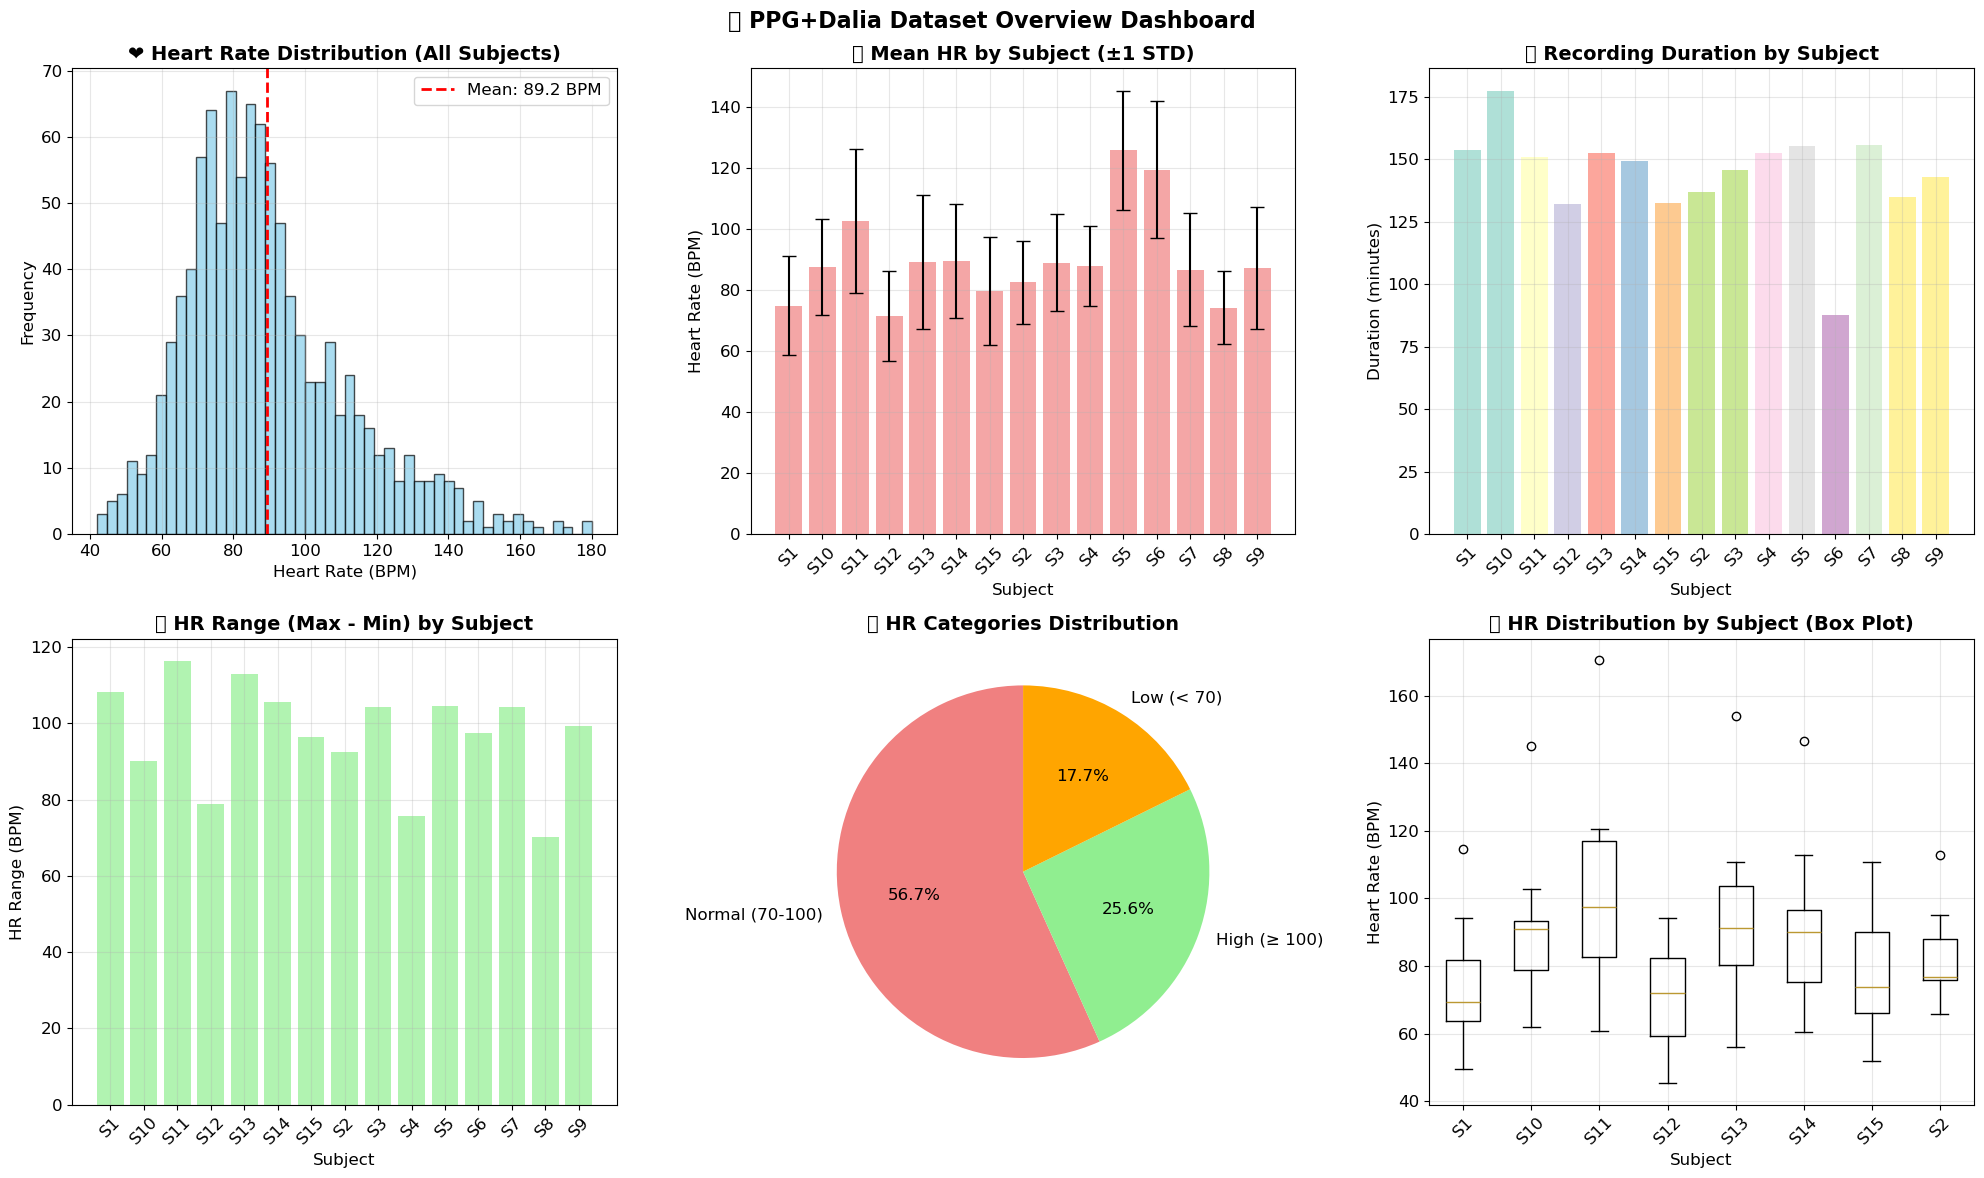
\includegraphics[width=1\textwidth]{Figures/Distribution PPG.png}
    \caption{Tableau de bord de la distribution des variables du dataset PPG+Dalia : fréquence cardiaque, durée d’enregistrement, catégories}
    \label{fig:Dist_dashboard}
\end{figure}



\subsubsection{Emotions dataset for NLP}

Pour le jeu de données Emotions, la distribution des différentes classes d’émotions est un facteur important pour l’équilibre de l’apprentissage. La figure~\ref{fig:dist_emotions_train} montre la répartition initiale des étiquettes d’émotions dans le corpus d’entraînement.

La distribution initiale est la suivante :
\begin{itemize}
    \item joy : 5362
    \item sadness : 4666
    \item anger : 2159
    \item fear : 1937
    \item love : 1304
    \item surprise : 572
\end{itemize}

\begin{figure}[H]
    \centering
    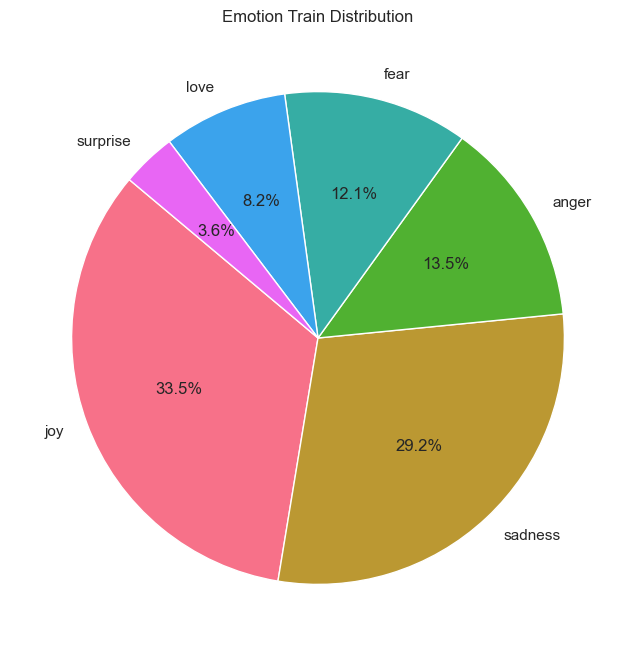
\includegraphics[width=0.6\textwidth]{Figures/emtion_train_distribution.png}
    \caption{Distribution initiale des classes d’émotions dans le dataset d’entraînement}
    \label{fig:dist_emotions_train}
\end{figure}

On constate un déséquilibre important entre les différentes classes. Pour garantir un apprentissage équitable du modèle, nous avons procédé à un équilibrage du dataset.

Cette analyse permet de vérifier l’absence de biais majeur et d’anticiper d’éventuels déséquilibres à corriger lors de l’entraînement des modèles.

\subsection{Préparation et prétraitement des données}

Le prétraitement des données est une étape clé pour garantir la qualité des analyses et la performance des modèles. Les étapes suivantes ont été réalisées pour chaque jeu de données, en s’appuyant sur des scripts Python dédiés.

\paragraph{Pour le dataset PPG+Dalia :}
\begin{itemize}
    \item \textbf{Chargement automatique et vérification des fichiers sujets} grâce à une classe dédiée (\texttt{PPGDaliaDataExplorer}), permettant de parcourir et d’importer tous les fichiers \texttt{.pkl} du dossier de données.
    \item \textbf{Extraction des signaux physiologiques} : récupération des signaux PPG (BVP), ECG, EDA, température, ainsi que des labels de fréquence cardiaque (HR) pour chaque sujet.
    \item \textbf{Synchronisation et nettoyage} : gestion des valeurs manquantes, conversion des clés binaires, suppression des signaux incomplets ou aberrants.
    \item \textbf{Analyse de structure et statistiques globales} : calcul automatique du nombre de sujets, de la durée totale, des types de signaux disponibles, de la distribution des valeurs de HR, etc.
    \item \textbf{Découpage en fenêtres temporelles} : segmentation des signaux bruts en fenêtres de taille fixe (par exemple 10 secondes, soit 640 échantillons à 64 Hz) pour l’extraction de caractéristiques locales.
    \item \textbf{Filtrage passe-bande} : application d’un filtre numérique (0.5–4 Hz) sur le signal PPG pour éliminer le bruit et les artefacts.
    \item \textbf{Extraction de caractéristiques avancées} : calcul de descripteurs temporels (moyenne, médiane, écart-type, etc.), fréquentiels (énergie spectrale, fréquence dominante, etc.), et ajout de variables démographiques synthétiques (âge, genre, fitness).
    \item \textbf{Construction des labels de classification} : attribution d’une classe (basse, normale, élevée) à chaque fenêtre selon la médiane du HR de référence.
    \item \textbf{Équilibrage intelligent des classes} : rééchantillonnage pour obtenir un nombre similaire de fenêtres par classe, avec sur-échantillonnage contrôlé si besoin.
\end{itemize}

\paragraph{Pour le dataset Emotions (NLP) :}
\begin{itemize}
    \item \textbf{Chargement des données} : Import des fichiers \texttt{train.csv}, \texttt{val.csv} et \texttt{test.csv} dans des DataFrames pandas.
    \item \textbf{Analyse et visualisation de la distribution des émotions} : Comptage des occurrences de chaque émotion et visualisation par diagramme circulaire pour détecter les déséquilibres.
    \item \textbf{Filtrage des classes minoritaires} : Suppression des émotions trop peu représentées (\textit{love}, \textit{surprise}) dans tous les ensembles pour garantir la robustesse du modèle.
    \item \textbf{Équilibrage du dataset d'entraînement} : Sous-échantillonnage ou sur-échantillonnage de chaque classe pour obtenir le même nombre d’exemples par émotion (par la méthode du tirage aléatoire avec ou sans remise).
    \item \textbf{Préparation des données textuelles et des labels} : Extraction des textes et des étiquettes d’émotion pour chaque ensemble (train, validation, test).
    \item \textbf{Encodage des labels} : Transformation des émotions en labels numériques à l’aide de \texttt{LabelEncoder}.
    \item \textbf{Tokenisation et vectorisation} : Création d’un \texttt{Tokenizer} Keras (vocabulaire limité à 10\,000 mots), conversion des textes en séquences d’indices, puis padding à une longueur fixe (50 tokens).
    \item \textbf{Conversion des labels en one-hot} : Transformation des labels numériques en vecteurs binaires pour l’apprentissage supervisé.
    \item \textbf{Vérification des dimensions finales} : Contrôle du vocabulaire, de la longueur des séquences et du nombre de classes pour garantir la cohérence des entrées du modèle.
\end{itemize}

\begin{center}
    
\includegraphics[height=1.4cm]{Figures/jupyter.png}\\
    \textit{Toutes ces étapes de préparation et de prétraitement ont été réalisées et automatisées dans un notebook \textbf{Jupyter}, assurant un pipeline reproductible et interactif.}
\end{center}

Ce pipeline de préparation garantit la qualité, la diversité et la pertinence des données utilisées pour l’entraînement et l’évaluation des modèles d’IA intégrés dans MindCare-AI.

\section{Modélisation et évaluation}

Cette section présente la démarche de modélisation des différents modules d’intelligence artificielle intégrés dans MindCare-AI, ainsi que l’évaluation expérimentale des performances obtenues. Deux axes principaux sont abordés : la classification de la fréquence cardiaque à partir des signaux physiologiques (PPG+Dalia) et la classification des émotions à partir de textes (dataset Emotions). Enfin, l’intégration de ces modèles dans le chatbot est discutée.

\subsection{Modélisation pour la classification de la fréquence cardiaque (PPG+Dalia)}

\paragraph{Choix des modèles et pipeline}
Pour la tâche de classification de la fréquence cardiaque, plusieurs modèles d’apprentissage automatique ont été testés, notamment : \textit{Random Forest}, \textit{Gradient Boosting}, \textit{SVM}, \textit{MLP}, et différentes variantes d’arbres de décision. Le pipeline inclut la normalisation des caractéristiques, la sélection de variables pertinentes et l’entraînement sur des fenêtres temporelles extraites du signal PPG.

\paragraph{Entraînement et validation croisée}
Les modèles ont été entraînés sur un jeu de données équilibré, avec une validation croisée pour évaluer la robustesse. Les métriques utilisées incluent la précision, le rappel, la F1-score et la matrice de confusion pour chaque classe (basse, normale, élevée).

\paragraph{Résultats}
Le meilleur modèle obtenu  Gradient Boosting  atteint une précision de \textbf{96,7\%} sur le jeu de test, avec une bonne capacité à distinguer les trois classes de fréquence cardiaque. Les résultats détaillés sont présentés dans le tableau~\ref{tab:hr_classification_results} et la figure~\ref{fig:hr_confusion_matrix}.

% Exemple de tableau de résultats
\begin{table}[H]
    \centering
    \caption{Performances des modèles de classification de la fréquence cardiaque}
    \begin{tabular}{lcccc}
        \hline
        \textbf{Modèle} & \textbf{Accuracy} & \textbf{F1-score} & \textbf{Overfit} \\
        \hline
        Gradient Boosting & 0.967 & 0.967 & 0.033 \\
        Decision Tree     & 0.683 & 0.689 & 0.183 \\
        Random Forest     & 0.867 & 0.867 & 0.112 \\
        XGBoost           & 0.933 & 0.933 & 0.067 \\
        SVM               & 0.8 & 0.81 & 0.112 \\
        \hline
    \end{tabular}
    \label{tab:hr_classification_results}
\end{table}

\begin{figure}[H]
    \centering
    \includegraphics[width=0.6\textwidth]{Figures/confusion matrix.png}
    \caption{Matrice de confusion Gradient Boosting HR}
    \label{fig:hr_confusion_matrix}
\end{figure}

\subsection{Modélisation pour la classification des émotions (NLP)}

\paragraph{Architecture du modèle}
Pour la classification des émotions, un modèle de deep learning basé sur un réseau de neurones convolutionnel (CNN) a été développé. Le pipeline comprend la tokenisation des textes, le padding, l’encodage des labels et l’entraînement du modèle sur le dataset équilibré.

\paragraph{Entraînement et évaluation}
Le modèle a été entraîné sur l’ensemble d’entraînement, avec validation sur un ensemble séparé. Les performances sont évaluées en termes d’accuracy, de F1-score et de matrice de confusion.

\paragraph{Résultats}
Le modèle atteint une précision de \textbf{94.24\%} sur le jeu de test, avec une bonne capacité à distinguer les principales émotions (joie, tristesse, colère, peur). Les résultats sont illustrés dans la figure~\ref{fig:emotion_confusion_matrix}.

\begin{figure}[H]
    \centering
    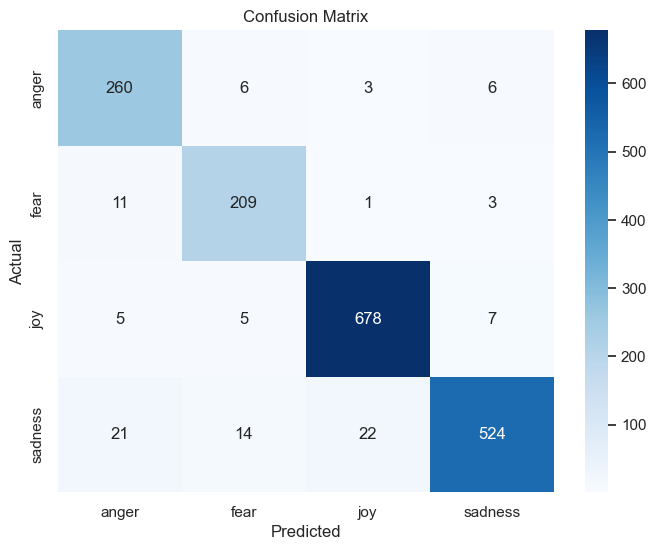
\includegraphics[width=0.6\textwidth]{Figures/matrice_emotion.png}
    \caption{Matrice de confusion du modèle de classification des émotions}
    \label{fig:emotion_confusion_matrix}
\end{figure}

\subsection{Intégration et évaluation dans le chatbot}

Les modèles de classification de la fréquence cardiaque et des émotions ont été intégrés au sein du chatbot MindCare-AI. L’évaluation de l’expérience utilisateur a montré que le système est capable de fournir des retours personnalisés, des conseils adaptés et d’améliorer le suivi du bien-être mental de manière interactive et sécurisée.

\paragraph{Limites et perspectives}
Parmi les principales limites identifiées figurent la taille relativement restreinte des jeux de données, la variabilité inter-individuelle des signaux physiologiques, ainsi que la nécessité d’une validation clinique plus approfondie. Les perspectives d’amélioration incluent l’augmentation du volume de données, l’intégration de signaux physiologiques supplémentaires et l’optimisation continue des modèles d’intelligence artificielle afin d’accroître la robustesse et la pertinence des recommandations fournies par le système.


\chapter{Réalisation }
\begingroup
%\parindent=0.2em
\etocsettocstyle{\rule{\linewidth}{\tocrulewidth}\vskip0.5\baselineskip }{\rule{\linewidth}{\tocrulewidth}}
\localtableofcontents 
\endgroup
\newpage
\section{Introduction}

\section{Environnement du developpement }
\section{Présentation des interfaces du générateur des test unitaires}
\section{Exemple d'exécutions }

\section{Conclusion}
In this chapter, we proposed two novel approaches ...
\chapter*{Conclusion générale}
\thispagestyle{fancy}
\addcontentsline{toc}{chapter}{Conclusion générale}

Ce projet de fin d'études, réalisé au sein de la société Mobelite, a permis de développer avec succès MindCare-AI, une solution innovante d'accompagnement en santé mentale qui démontre concrètement la faisabilité d'une approche intégrée combinant développement mobile moderne et intelligence artificielle avancée. L'analyse approfondie du contexte de la santé mentale digitale et l'identification précise des besoins utilisateurs ont guidé nos choix technologiques et méthodologiques, nous permettant de concevoir une architecture robuste capable de supporter les modules d'intelligence artificielle les plus exigeants.

La méthodologie de développement adoptée, structurant le projet en deux releases complémentaires suivant les principes agiles de Scrum et la rigueur scientifique de CRISP-DM, s'est révélée particulièrement efficace pour gérer la complexité technique tout en maintenant une approche centrée utilisateur. Cette approche duale nous a permis d'établir d'abord des fondations solides avec la Release 1, puis de les transformer en solution véritablement intelligente avec la Release 2, garantissant ainsi une progression maîtrisée vers l'excellence technique.

L'implémentation de la Release 1 a établi les fondations technologiques indispensables avec un système d'authentification sécurisé utilisant JWT et bcrypt, une architecture MVC modulaire facilitant l'évolutivité, un Home Screen personnalisé avec métriques temps réel, un assistant conversationnel empathique intégrant des évaluations psychologiques validées, et une interface d'analyse rPPG préparatoire avec détection faciale intelligente. Ces quatre sprints successifs ont livré une application mobile complète et immédiatement utilisable, validant nos choix architecturaux et préparant parfaitement l'intégration des capacités d'intelligence artificielle.

La Release 2 a transformé cette base solide en solution véritablement révolutionnaire par l'intégration de modules d'IA performants développés selon la méthodologie CRISP-DM rigoureuse. L'estimation rPPG des signes vitaux atteignant une précision exceptionnelle de 96.7%, la détection des émotions textuelles avec 94.24% d'accuracy, le chatbot adaptatif intelligent et le système de recommandations personnalisées dynamiques illustrent la maturité technique atteinte et positionnent MindCare-AI comme une référence dans l'écosystème de la santé mentale assistée par l'intelligence artificielle.

Les objectifs initiaux ont été largement dépassés avec une détection précoce et précise d'indicateurs de stress, un accompagnement personnalisé disponible 24/7, et une expérience utilisateur fluide intégrant harmonieusement les capacités d'IA avancées dans l'interface mobile native. La validation technique confirme la robustesse de l'architecture hybride combinant React Native et Node.js pour l'application mobile avec Python et TensorFlow pour les modules d'intelligence artificielle spécialisés, démontrant la pertinence de nos choix technologiques initiaux.

Les perspectives d'évolution identifiées ouvrent des horizons prometteurs : à court terme, l'enrichissement des datasets et l'optimisation des modèles permettront d'améliorer encore les performances, tandis qu'à moyen terme, l'extension vers d'autres paramètres physiologiques, l'intégration de capteurs wearables et la validation clinique approfondie transformeront MindCare-AI en écosystème complet de santé mentale digitale. Ce travail démontre ainsi le potentiel transformateur de l'intelligence artificielle au service du bien-être humain et établit les bases d'une nouvelle génération de solutions d'accompagnement psychologique personnalisé et accessible.
\addcontentsline{toc}{chapter}{Bibliographie}
\bibliographystyle{unsrt}
\bibliography{biblio}
\end{document}